\section{A two-bridge estimate and polygon shape mass}\label{c2:two-bridge}

To localize the cylinder partition function in the plane, we need a
positive bound on large polygon shapes. We obtain it by cutting a polygon
at its extreme rows and estimating the resulting pair of disjoint bridges.
The boundary inputs are \(h(d)\asymp d^{-5/4}\) and
\(B(R)\asymp R^{-1/4}\); write \(p=1/4\). The independent cylinder
calculation will enter only when we pass from shapes to nesting.

We work in the same horizontal strip as in the boundary part, of admissible physical height \(R=(3/2)H\), \(H\) a positive integer (bottom line at vertical coordinate \(-1/2\)). Index each line of ports by increasing integers. Thus bottom index \(j\) has horizontal coordinate \(j|U|\), top index \(j\) has coordinate \((j+H/2)|U|\). The letter \(x\) for weights is again the critical vertex weight. Orient bridges from bottom to top; their turning phase \(e^{\mathrm i sW}\) is 1, by enclosing any particular path in a large bounded cut strip and using the turn rule of \eqref{c2:eq-1}. Disjoint bridges with given sets of endpoints must match in increasing order, by planarity. Use
\[
 \sigma=\sum_{d\ge1}h(d)=\frac{1}{2\cos r},\qquad
 Q(n)=\sum_{d\ge1}\min(d,n)h(d)\asymp n^{1-p},\qquad
 B=B(R)\asymp R^{-p}.
\]
These are the half-plane and strip bounds already proved (in particular \(h(d)\asymp d^{-1-p}\), giving the estimate on \(Q\) by summation). \(B\) is the total strip bridge mass from one fixed bottom port. For tuple weights specified only by successive gaps on each wall we always \textbf{sum over relative horizontal offset}, i.e. fix the first bottom site and sum the first top index over all integers. Translating both lists by \(U\) reindexes, so one could equivalently fix a top base. Let \(f_{l,k}\) be the total mass \(x^{\#\text{vertices}}\) of disjoint pairs with bottom gap \(l\ge1\) and top gap \(k\ge1\) in this convention. Independent-bridge bounds apply, e.g. \(\sum_{k\ge1} f_{l,k}\le B^2\).

\begin{proposition}[Adjacent bridges and polygon shapes]
\label{prop:adjacent-bridges-shapes}
For an admissible strip of height \(R\), let \(F(R)=f_{1,1}\) be the
critical mass of pairs of vertex-disjoint bridges with adjacent endpoints
on each wall, fixing the first bottom port and summing the first top port.
For a full-plane simple polygon \(\gamma\), let \([\gamma]\) denote its
unrooted, unoriented translation class under the lattice generated by
\(U,V\). There is an absolute constant \(C\) such that
\[
 F(R)\le CR^{-3},\qquad
 \sum_{\substack{[\gamma]\\L\le\diam\gamma<2L}}x^{|\gamma|}
 \le CL^{-2}\qquad(L\ge1).
\]
\end{proposition}

\begin{proof}
We first gain adjacency at one wall, then at the other, by moving a vacant
source among existing ordered bridges. The last step cuts a polygon at
its two extreme rows and recovers it from the resulting bridge pair.

\subsection{Vacancies among ordered bridges}
An extra bottom source can either form a new bridge or an arch; the arch
mass lost to the existing bridges measures the obstruction. Moving the
extra source among the bottom roots cancels its first collisions with
those bridges.

Here is the precise identity. Initially fix the offset and all sites: take an increasing list of bottom sites and an increasing list of top sites with one fewer element. For each choice of one vacant bottom site consider disjoint existing bridges from the other sites to the top list in order, and label these cases by consecutive integers \(j\) from left vacancy to right vacancy (any starting integer). For each existing tuple take the bare critical arch masses in the full upper half-plane from the vacancy to the bottom line, separately to its left and its right. Let \(L_j,R_j\) be the masses \textbf{lost} in these two directions upon demanding that the arch stay in the strip and be disjoint from the existing paths (including distinct endpoints), weighted and summed over the existing tuples. Let \(T_j\) be the weight of the existing tuples with an additional disjoint bridge from the vacancy to any free top port. Then
\begin{equation}
 \sum_j e^{(2j-2)\mathrm i r}
       \big(e^{\mathrm i r} L_j+e^{-\mathrm i r}R_j-T_j\big)=0.              \label{c2:eq-B1}
\end{equation}

To prove it, cut the strip first by distant sides of the convex-polygon exhaustion in \eqref{c2:eq-1}, restricting also the existing tuples to that polygon and giving each path its complex turn weights. Explore non-backtracking from the vacancy as in \eqref{c2:eq-1}, stopping at an exit, a self-repeat or on hitting any occupied vertex (in the last two cases before another turn). Its total weight is one. Self-repeat terms cancel by reversing the newly closed loop as before. A hit of an existing bridge comes along its unused edge at the branch vertex. This can be only a bridge with a bottom source neighboring the vacancy in the list: an intervening disjoint bottom-to-top bridge separates them. Switch the two initial legs, i.e. pass to the neighboring vacancy case by retaining the target leg of the hit bridge for the new through path and using its old initial leg now as the stopped exploration. All paths satisfy the same simplicity/disjointness requirements up to this first hit, and this operation is a bijection of collision terms. 

The cyclic order of the three rays towards left source, right source and top target is counterclockwise (the order at the boundary for three disjoint legs). Thus the through turn for the left vacancy case is \(-\pi/3\), and for the right vacancy case \(+\pi/3\); all other directed turns on the legs agree, with unchanged magnitude of weight. The ratio from left to right including the coefficients in \eqref{c2:eq-B1} is \(e^{\mathrm i(2r+2r/3)}=-1\), giving cancellation. 

On exhaustion, exits on the receding sides cost vanishing mass even ignoring avoidance, by half-plane saturation for that vacancy start, with existing weights bounded by products of \(B\)'s. Existing bridges have phase 1 and allowed arch exits on the bottom have phases \(e^{\mathrm i r},e^{-\mathrm i r}\) to left, right. These disjoint exit terms pass to the strip limit with finite positive masses (times the indicated phases). After the collision cancellation their weighted sum over vacancy cases equals the similarly weighted sum of the bare existing-tuple masses by the exploration total. Subtract the exit terms from the independent half-plane arch comparison (mass \(\sigma\) in each direction per tuple, so total with its phases one) to get \eqref{c2:eq-B1}. We may also sum the identity over offsets and the top gap choices used below: the absolute masses \(L_j,R_j,T_j\) are bounded by independent \(\sigma,\sigma,B\) times existing bridge masses, and summed existing lists by independent bridges from fixed bottom starts.

Multiplying \eqref{c2:eq-B1} by \(e^{\mathrm i r}\), taking imaginary parts and dividing by \(\sin(2r)>0\), the coefficient triples on \(L_j,R_j,T_j\) for the cases needed are
\[
\begin{array}{c|rrr}
 j & L_j & R_j & T_j\\ \hline
 -1&-1&\sqrt2&-b_*\\
 0&0&-1&a_*\\
 1&1&0&-a_*\\
 2&-\sqrt2&1&b_*
\end{array}
\qquad
 a_*=\frac{\sin r}{\sin(2r)}=\sigma,\qquad
 b_*=\frac{-\sin(3r)}{\sin(2r)},\qquad a_*>b_*>0.
\]

\subsection{A positive estimate for summed arch losses}
The individual differences of left and right losses below can have either
sign. We use them only after summing the vacancy over an interval, when
symmetry of the lost-arch kernel supplies a positive lower bound.

We will place vacancies outside a fixed weighted ensemble \(\mathcal E\) of one or more existing ordered strip bridges (fixed bottom list, possibly summed top choices), writing \(|\mathcal E|\) for its mass. For insertion \(i\ge1\) sites to the right of the rightmost bottom root let \(D^{\rm right}_{\mathcal E}(i)=\sqrt2 L-R'\), where \(L,R'\) are the same left and right losses integrated over \(\mathcal E\). For insertion \(i\) sites to the left of the leftmost root set \(D^{\rm left}_{\mathcal E}(i)=\sqrt2 R'-L\). For either convention use the outward integer coordinate from the extreme root (0 there, positive outwards), and write \(\mathscr K(i,j)\) for the integrated lost arch weight between two distinct sites in this coordinate, so it is symmetric and \(\mathscr K(i,j)\le h(|i-j|)|\mathcal E|\). For \(i>0,\ j\le0\) this last bound is an equality: any such arch staying in the strip is blocked by a bottom-to-top bridge at the extreme root. With \(I_{\mathcal E}(n)=\sum_{1\le i<j\le n}\mathscr K(i,j)\) in the chosen convention and \(c_0=\sqrt2-1\), it follows that
\begin{equation}
 c_0\big(Q(n)|\mathcal E|+I_{\mathcal E}(n)\big)
 \ \le\ \sum_{i=1}^n D_{\mathcal E}(i)
 \le\ \sqrt2 Q(n)|\mathcal E|+c_0 I_{\mathcal E}(n).                     \label{c2:eq-B2}
\end{equation}
Indeed the within-interval terms have net coefficient \(c_0\). Across the edge towards the bridges the loss contributes \(\sqrt2 Q(n)|\mathcal E|\), while across the far edge the negative term costs at most \(Q(n)|\mathcal E|\).

\subsection{Adjacency at one wall}
Take now three bottom sites \(w,w+1,w+1+l\), vacancies indexed \(0,1,2\), and two top sites \(s',s'+k\) (\(l,k\ge1\)), integrating \(s'\) over indices (including in the \(T_j\)'s below). Let \(\mathcal F_k\) be the existing ensemble for vacancy 2 (mass \(f_{1,k}\), independent of \(l\)). Losses \(R_0,L_1\) are full in their directions because the consecutive bottom pair allows no endpoint in between and a bridge blocks crossing. Thus \eqref{c2:eq-B1} with the coefficient table gives
\begin{equation}
 \sigma(f_{l+1,k}-f_{l,k})=D^{\rm right}_{\mathcal F_k}(l)-a_*T_0+a_*T_1-b_*T_2.       \label{c2:eq-B3}
\end{equation}
When summed over all \(k\ge1\), the \(T_0,T_1\) masses are equal (each counts the triples with those bottom roots and all increasing top choices; the extra top port is first, respectively second). Also \(T_2\le B f_{1,k}\). Sum \eqref{c2:eq-B3} over \(k\) and \(1\le l\le m=\lfloor\delta R\rfloor\) with small constant \(\delta>0\), for large \(R\). By \eqref{c2:eq-B2} the right side is at least \((c_0 Q(m)-b_*mB)\sum_k f_{1,k}\). The telescoped left side is at most \(\sigma B^2\). We can make \(mB/Q(m)\) small since it is \(O(\delta^p)\); hence
\begin{equation}
 \sum_k f_{1,k}\lesssim B^2/Q(m),\qquad
 \sum_k f_{k,1}\lesssim B^2/Q(m).                                          \label{c2:eq-B4}
\end{equation}
For the second inequality exchange top and bottom. Explicitly the lattice strip symmetry on horizontal and vertical coordinates is
\((u,v)\mapsto(u+H|U|/2,(3/2)H-1-v)\), sending \(\mathbf a_{jk}\) to \(\mathbf b_{j+k,H-1-k}\) and \(\mathbf b_{jk}\) to \(\mathbf a_{j+k+1,H-1-k}\); offsets reindex.

\subsection{Adjacency at both walls}
The estimates in \eqref{c2:eq-B4} impose adjacency at one wall while
summing the gap at the other. Our target is the sharper individual term
\(F=f_{1,1}=O(R^{-3})\). To gain that second adjacency constraint, we now
compare three-bridge ensembles by moving a vacancy among four bottom
sites. The resulting two-variable telescoping identity will feed back
into the first vacancy relation.

Write \(f_l=f_{l,1}\), \(F=f_1\), \(\mathcal F=\mathcal F_1\), \(D(l)=D^{\rm right}_{\mathcal F}(l)\). Use triple masses \(g_l,A_l\) for bottom gaps \(1,l\); \(g_l\) uses top gaps \(t,1\) summing \(t\ge1\), and \(A_l\) uses \(1,t\) summing \(t\ge1\). Denote the latter ensemble on bottom roots \(w,w+1,w+1+l\) by \(\mathcal A_l\). For \(k=1\) in \eqref{c2:eq-B3} there is no intermediate top site, so
\begin{equation}
 \sigma(f_{l+1}-f_l)=D(l)-a_* g_l-b_* A_l,\qquad A_l\le BF.                 \label{c2:eq-B5}
\end{equation}

Use four bottom sites \(w-k,w,w+1,w+1+l\), \(k,l\ge1\), vacancy indices \(-1,0,1,2\), and three top sites with gaps \(1,t\) summing offset and \(t\ge1\). Write \(K_{k,l}\) for the triple mass with bottom gaps \(k,l\) and those summed top choices. The existing ensemble in case 2 has bottom roots \(w-k,w,w+1\); call it \(\mathcal E_k\). Its mass equals \(g_k\) by left-right reflection (reversing both lists). We have also the left-right lattice symmetry on a strip, \((u,v)\mapsto(-u,v)\), with shifts of base indices absorbed by the offset sum. Case \(-1\) has existing ensemble \(\mathcal A_l\). Again the consecutive bottom pair gives full losses in cases 0 to right and 1 to left. Thus
\begin{equation}
\begin{split}
 \sigma(K_{k,l+1}-K_{k+1,l})
 &=D^{\rm right}_{\mathcal E_k}(l)-D^{\rm left}_{\mathcal A_l}(k)
       +b_*T_{-1}-a_*T_0+a_*T_1-b_*T_2\\
 &\ge D^{\rm right}_{\mathcal E_k}(l)-D^{\rm left}_{\mathcal A_l}(k).
\end{split}                                                               \label{c2:eq-B6}
\end{equation}
Indeed \(T_0=0\) (no extra port in the consecutive top gap); \(T_1=T_2\) after the \(t\) integration (both count all ordered quadruples with the first top gap 1), and \(a_*\ge b_*\).

For two vacancy endpoints both to the left of \(w\), the kernel \(\mathscr K\) for \(\mathcal A_l\) is bounded by \(B\) times that for \(\mathcal F\) on the left. In fact an arch there which stays in the strip disjoint from the first two bridges remains on their left and cannot touch the third (crosscut separation); for any fixed first two forming a tuple in \(\mathcal F\), possible third bridges cost at most \(B\). Use the leftward coordinate for both ensembles. The positive
kernel comparison gives
\[
 I_{\mathcal A_l}(n)\le B I_{\mathcal F}^{\rm left}(n),
 \qquad |\mathcal A_l|=A_l\le BF.
\]
The upper and lower bounds in \eqref{c2:eq-B2} now imply
\[
\begin{aligned}
 \sum_{k=1}^n D^{\rm left}_{\mathcal A_l}(k)
 &\le B\big(\sqrt2 Q(n)F+c_0 I_{\mathcal F}^{\rm left}(n)\big)\\
 &\le \frac{\sqrt2}{c_0}B
       \sum_{k=1}^n D^{\rm left}_{\mathcal F}(k)
  =\frac{\sqrt2}{c_0}B\sum_{k=1}^nD(k).
\end{aligned}
\]
The last equality uses left-right reflection of the adjacent-pair ensemble.
This argument compares interval sums of the signed losses; it makes no
pointwise comparison of the individual \(D\)'s.

Sum \eqref{c2:eq-B6} over \(1\le k,l\le n\). The positive boundary sums remaining on telescoping the \(K\)'s are bounded by
\(\sum_{k=1}^n K_{k,n+1}+\sum_{l=1}^n K_{1,l}\le B(\sum_k f_k+nF)\) by dropping the last bridge. By \eqref{c2:eq-B2} and the preceding comparison we get
\begin{equation}
 c_0 Q(n)\sum_{k=1}^n g_k
 \le \sigma B\big(\sum_k f_k+nF\big)+C Bn\,D_\Sigma(n),
 \qquad D_\Sigma(n):=\sum_{l=1}^n D(l)\ge c_0 Q(n)F.                       \label{c2:eq-B7}
\end{equation}
It remains to close the two estimates: \eqref{c2:eq-B5} bounds the
summed losses by triple masses, and \eqref{c2:eq-B7} bounds those triple
masses by the summed losses with a small coefficient. Set
\(S_f=\sum_{k\ge1}f_k\). Summing \eqref{c2:eq-B5} and then applying
\eqref{c2:eq-B7} gives, for \(m/2\le n\le m\),
\[
\begin{aligned}
 D_\Sigma(n)
 &\le \sigma f_{n+1}+a_*\sum_{l=1}^n g_l+b_*nBF\\
 &\le \sigma f_{n+1}
   +C\frac{B S_f}{Q(n)}
   +C\frac{BnF}{Q(n)}+C\frac{Bn}{Q(n)}D_\Sigma(n)+b_*nBF.
\end{aligned}
\]
Since \(Q(n)\ge c>0\) and \(F\le D_\Sigma(n)/(c_0Q(n))\), all the
terms in the second line containing \(F\) or \(D_\Sigma(n)\) are at most
\(C'BnD_\Sigma(n)/Q(n)\). The coefficient is \(O(\delta^p)\), uniformly
for these \(n\). Choose \(\delta\) once so that it is less than one half.
Absorbing it and using \(Q(n)\asymp Q(m)\) yields
\[
 Q(m) F\lesssim f_{n+1}+B\sum_k f_k/Q(m)
 \qquad(m/2\le n\le m).
\]
Average in \(n\), then use \eqref{c2:eq-B4}:
\begin{equation}
 F\ \lesssim\ Q(m)^{-1}\big(m^{-1}+B/Q(m)\big)\, B^2/Q(m)
 \ =\ O(R^{-3}).                                                          \label{c2:eq-B8}
\end{equation}

\subsection{Cutting polygon shapes into adjacent bridges}
It follows that the total critical mass of translation classes of full-plane simple polygons of Euclidean diameter in \([L,2L)\) is \(O(L^{-2})\) as \(L\to\infty\). Here a polygon is an unoriented unrooted simple lattice cycle \(\gamma\) of weight \(x^{|\gamma|}\) (vertex count \(|\gamma|\)), and translations are by the lattice generated by \(U,V\). The estimate is on translation classes, so we retain an injective
encoding by choosing the leftmost vertex at each extreme height. One of the three lattice
axes gives a height projection span comparable to \(L\); sum over these choices and use a \(120^\circ\)-multiple lattice rotation to make it the usual vertical height. Minimum vertices of the polygon in this direction are all of type \(\mathbf a\) (a \(\mathbf b\) has only one upward edge), and maximum vertices all of type \(\mathbf b\), both using their two slanted edges. At the leftmost minimum \(\mathbf a_{jk}\) delete its polygon edge to the upper-left neighbor \(\mathbf b_{j-1,k}\); attach a downward exterior half-edge from \(\mathbf a_{jk}\) to a port, and at the unused minimum-row vertex \(\mathbf a_{j-1,k}\) attach its downward half-edge to the adjacent port and the edge to \(\mathbf b_{j-1,k}\). Similarly at the leftmost maximum \(\mathbf b_{dh}\) delete the edge to the lower-left neighbor \(\mathbf a_{d,h}\); attach an upward exterior half-edge from \(\mathbf b_{dh}\) to a port, and at the unused maximum-row vertex \(\mathbf b_{d-1,h}\) attach its upward half-edge to the adjacent port and the edge to \(\mathbf a_{d,h}\).

For these large spans the changes are apart. Cutting the two edges on a simple cycle gives two paths each running from one cut to the other; the attachments now make two vertex-disjoint bottom-to-top bridges of a strip, in order by planarity, with adjacent endpoints at each wall. Its height is the vertex span plus one, hence admissible and comparable to \(L\). Translate to fix the bottom neighboring pair (left added vertex at \(\mathbf a_{00}\)). The resulting pair is counted by \(F\) at that height, with joint weight \(x^{|\gamma|+2}\); the encoding on translation classes for that direction is injective (trim the added left vertex on each wall and restore the specified edges). There are \(O(L)\) height choices, proving the claim by \eqref{c2:eq-B8}.
\end{proof}

In particular on a full cylinder of horizontal period \(NU\), contractible simple polygons enclosing a specified point, with planar lift diameter in a dyad \([L,2L)\) where \(L\gtrsim N\), cost \(O(N/L)\) total positive mass. Lift a polygon to its planar closed copy; for any translation class there are at most \(O(NL)\) placements modulo the cylinder period which can enclose the point (vertical translation has \(O(L)\) choices to put its height in the span, horizontal index at most \(N\) modulo period). This bound sums to \(O(1)\) on dyads above any fixed constant times \(N\).

\section{Winding polygons on the cylinder}\label{c2:winding}

We also need a uniform single-loop cost bound for the noncontractible polygons that separate two antipodal gaps. Work on the full cylinder of period \(2nU\), \(n\ge3\), and first restrict polygons to a strip of finitely many whole consecutive layers as above on this cylinder. A winding polygon is a simple polygon noncontractible on the cylinder (unoriented and unrooted). For winding polygons write \(\eta<\gamma\) if they are disjoint and \(\eta\) is below \(\gamma\), i.e. on its side towards the lower end. Any two disjoint ones are ordered. These separation conventions follow for example by mapping the cylinder in horizontal and vertical coordinates \(u,v\) to the punctured plane by
\(\exp(2\pi \mathrm i(u+\mathrm i v)/(2n|U|))\). A winding simple curve surrounds 0 in that plane, with upper end on the bounded side; it winds once up to sign by Jordan curve separation (index of a simple closed curve). The positive traversal (lift displacement \(+2nU\)) has lower side on its right.

Set \(t_0=2\cos(2\pi s/3)=\sqrt2\).
\begin{proposition}[Uniform mass of winding separators]
\label{prop:winding-separators}
On the honeycomb cylinder of period \(2nU\), \(n\ge3\), let \(f\) be a
point off the lattice edges and put \(f'=f+nU\). Then
\begin{equation}
 \sum_{\substack{\eta\ {\rm winding\ on\ full\ cylinder}\\
                 \eta\ {\rm separates}\ f,f'}} x^{|\eta|}
 \le 2/t_0.
 \label{c2:eq-C3}
\end{equation}
The polygons in this sum are simple, unrooted and unoriented.
\end{proposition}

\begin{proof}
We first work in a strip of finitely many complete layers. Exploration
excludes eigenvalue one for a matrix that records which winding polygons
can lie below one another. Adding layers continuously then places its
spectral radius below one. Finally, the two opposite assignments of
\(f,f'\) to the sides of a separator give two intersecting classes; their
equal masses are bounded by that spectral radius.

\subsection{A finite matrix and a deformation of the top row}
On the finite list of winding polygons in the strip consider the nonnegative matrix
\[
 A_{\gamma\eta}=t_0 w_\eta\,\mathbf1_{\{\eta\not<\gamma\}},
 \qquad w_\eta=x^{|\eta|}.
\]
Deform at the top layer by \(0\le\theta\le1\), replacing \(w_\eta\) by
\[
 w_\eta(\theta)=x^{|\eta|}\theta^{\,\#\{\text{topmost }\mathbf b\text{-row vertices on }\eta\}}
\]
(with zero exponent giving 1 for that factor), and call the corresponding matrix \(A(\theta)\).

Fix a bottom starting port. Explore non-backtracking with the complex transition weights of \eqref{c2:eq-1}, stopping on first repeat of a cylinder vertex before turning there, or at an exit. Modify only the turns upon arrival at a topmost \(\mathbf b\)-vertex (necessarily arriving from an internal edge below). Of the two choices, the transit to the other internal edge, of turn \(\tau_i=\pm\pi/3\), gets weight \(\theta x e^{\mathrm i s\tau_i}\); the upward exit, of opposite turn \(\tau_e\), gets weight \(1-\theta x e^{\mathrm i s\tau_i}\). Total outgoing weight stays one (the standard rule is recovered at \(\theta=1\)). Besides this full-strip experiment with flat top \(*\), run one for each winding ceiling \(\gamma\) by stopping also upon first hit of a vertex of that polygon, before turning there; then there can be no flat top exit before such a hit. Denote by \(S(\gamma)\) the real part of the ceiling hit terms, by \(S(*)\) the real part of flat top exit terms in the full experiment, and by \(D(\gamma),D(*)\) one minus the real part of the respective bottom exit sums, all with these same rules at fixed \(\theta\). The finite explorations give
\begin{equation}
 S(\gamma)=D(\gamma)-t_0\sum_{\eta<\gamma}w_\eta(\theta)S(\eta),
 \qquad
 S(*)=D(*)-t_0\sum_\eta w_\eta(\theta)S(\eta).                             \label{c2:eq-C1}
\end{equation}

\paragraph{Repeated vertices and loop turns.}
To verify the repeat contributions here, a first repeat has a simple stem reaching the attachment of a simple cylinder polygon along the third edge there. For a contractible loop the stem reaches from exterior (the bottom port is outside, toward the lower end); as in the plane its two loop orientations add turns \(\pm4\pi/3\) relative to the incoming stem, and cancel. For a winding loop \(\eta\) the stem reaches instead from its lower side. The closed positive traversal has net turn zero in the local lifted directions, with a turn \(+\pi/3\) at this attachment: the right-side local sector contains the unused third ray (from the lower side), so is the larger \(4\pi/3\) sector, corresponding to that positive turn. For the net turn assertion cut a lift at a minimum-height vertex of the polygon (type \(\mathbf a\) with both upward slants used, exiting upper-right in the positive traversal). Extend both ends straight down to a lower line. This makes a simple planar chord with positive horizontal displacement, going up from and down to the line, of total turn \(-\pi\) by closing clockwise on the line (two closing joins of \(-\pi/2\)); the two \(-\pi/3\) turns added at the endpoint copies replace the single cyclic \(+\pi/3\) turn. Thus the loop has turn zero as claimed. At the stem attachment the turn on actual positive departure from the incoming stem is \(-\pi/3\) instead of \(+\pi/3\); the two orientations therefore add relative turns \(-2\pi/3,+2\pi/3\).

All extra \(\theta\) factors from internal transits respect these calculations under reversal: a topmost \(\mathbf b\)-vertex cannot be the attachment (the stem arrives from inside there and three distinct internal edges would be required), and any passage on a loop there uses the two internal edges. Repeat histories with winding loop \(\eta\) are exactly first-hit stems to \(\eta\) followed by either traversal (the stem avoids it before that vertex and hence arrives along the unused edge). Under ceiling \(\gamma\) such loops necessarily satisfy \(\eta<\gamma\); conversely for any such \(\eta\) the stems to it from the bottom cannot previously hit \(\gamma\) by separation. The weight factor for the two added traversals together is \(t_0 w_\eta(\theta)\). This proves \eqref{c2:eq-C1} by taking real parts of the total-weight identities.

\paragraph{Positive flat exits and exclusion of eigenvalue one.}
Bottom arch exits have turns \(\pm\pi\) on lifting to plane chords, so still have nonnegative real weights (the modification only scales their prior internal transits by \(\theta\)). Under \(\gamma\) these arches are a subset of the flat experiment's arches, so \(D(\gamma)\ge D(*)\). Through bridges to the flat top would have total turn zero by lifting. Thus in a top exit term its prefix phase before the final turn is \(e^{-\mathrm i s\tau_e}\), with the extra nonnegative scaling for earlier top-row transits, and including the exit weight the resulting real factor is
\(\cos(\pi s/3)-\theta x\cos(2\pi s/3)\ge x>0\). A strictly ascending simple bridge with no earlier such transit exists even at \(\theta=0\). Hence \(S(*)>0\). From \eqref{c2:eq-C1} the real vector \(S=(S(\gamma))_\gamma\) satisfies
\begin{equation}
 (I-A(\theta))S=\big(S(*)+D(\gamma)-D(*)\big)_\gamma>0.                  \label{c2:eq-C2}
\end{equation}
The vector \(S\) need not have positive coordinates. Nevertheless
\(\rho(A(\theta))\ne1\): otherwise there is a nonnegative nonzero left eigenvector for eigenvalue 1, contradicting \eqref{c2:eq-C2}. To see that eigenvector fact directly for a finite nonnegative matrix (write it as \(A\)) of spectral radius 1, apply the resolvent of its transpose to the all-ones column at real \(z>1\); this is nonnegative by the power series. These columns must become unbounded as \(z\downarrow1\), since a bounded subsequential limit \(v\) would satisfy \(v=A^{\mathsf T}v+\mathbf1>0\), and diagonal scaling by \(v\) would give row sums strictly below one for the scaled transpose. Normalizing the unbounded columns and taking a limit yields the desired eigenvector.

\paragraph{Adding layers.}
Now induct by adding one strip layer at a time on top. At \(\theta=0\) any polygon using the added layer has zero modified weight (it must use a topmost \(\mathbf b\), since a new \(\mathbf a\) has only one edge below). Hence the columns for the new polygons vanish and the old-polygon submatrix is exactly the old matrix, so the spectral radius is the old one (zero initially; empty lists are harmless). Eigenvalues as a multiset, hence spectral radius, vary continuously with \(\theta\) (finite matrices, continuity of polynomial roots). By \eqref{c2:eq-C2} it follows inductively that \(\rho(A(1))<1\) in every such strip.

\subsection{Separators of two antipodal points}
The spectral bound now controls the positive mass of the loops we need.
Take any point \(f\) off the lattice edges on the cylinder and \(f'=f+nU\). Among winding polygons in the strip let \(\mathcal C\) be those with \(f\) on the lower side and \(f'\) on the upper, and \(\mathcal C'\) those with the opposite assignment. Half-period translation interchanges these classes, so both have the same total \(w\)-mass \(W_0\). Any opposite-class pair intersects by the ordering of disjoint winding curves. Therefore \(A=A(1)\) applied to the indicator vector of their union dominates \(t_0 W_0\) times that vector (cross-blocks are full), implying \(\rho(A)\ge t_0W_0\) by taking powers if \(W_0>0\). Consequently their combined mass is at most \(2/t_0\).
Exhausting vertically by whole-layer strips proves \eqref{c2:eq-C3}.
\end{proof}

\section{Planar nesting exponent and a bulk visit identity}\label{c2:nesting}

For a lattice face center \(f\) in the plane let \(Z_R(f)\) be the sum over collections of pairwise vertex-disjoint simple polygons all enclosing \(f\), with their vertices in the Euclidean ball of radius \(R\) about \(f\). Include the empty collection, and use product weight with \(2x^{|\gamma|}\) per polygon. We claim
\begin{equation}
 Z_R(f)=R^{z+o(1)},\qquad z=\frac1{12}.                                    \label{c2:eq-G1}
\end{equation}
The face centers are lattice-congruent by translations. In \(V_{n,n}(0)\) of the gluing identity (angle zero, polygon fugacity 2), choose \(f\) to be the midpoint in the seam gap before the initial block, i.e. a face center (up to translation we can take \(e_2/2+U/2\)), and \(f'=f+nU\), as points on the cylinder of period \(2nU\). By the contour estimate and the polygon interpretation, this positive separator partition sum is \(n^{1/6+o(1)}\).

The square of a planar nesting partition appears because a small
separator surrounds exactly one of the two cylinder marks. We show that
all other separators change the partition function by only a bounded
factor.

Fix \(0<c<|U|/3\). Any two planar collections counted in radius \(cn\) balls around lifts of \(f,f'\) project together to an allowed cylinder collection: the balls and their relevant period-translates are disjoint, and the polygons separate the two points. This is injective using the specified balls. Thus \(V_{n,n}(0)\ge Z_{cn}(f)^2\). 

Conversely a contractible separator encloses exactly one of the two points in its disk side, and lifts uniquely around the chosen lift of that point (the lifted polygon and its period translates have disjoint disks by simplicity; such translated bounded disks with disjoint boundaries cannot nest). Unless all vertices are in this \(cn\) ball, its planar lift diameter is at least \(cn\) since the enclosed point is in the convex hull. These large contractible separators have total single-polygon \(2x^{|\gamma|}\) mass \(O(1)\) by the cylinder consequence of Proposition~\ref{prop:adjacent-bridges-shapes}. Winding separators have bounded total mass by Proposition~\ref{prop:winding-separators}. Dropping all disjointness requirements on this large-or-winding group costs a partition factor at most the exponential of their total mass. Every remaining subcollection around either point lifts into its indicated ball as disjoint planar polygons. Together with the earlier injection, this gives
\begin{equation}
 Z_{cn}(f)^2\le V_{n,n}(0)\le e^C Z_{cn}(f)^2,
 \label{eq:disk-localization}
\end{equation}
where \(C\) is independent of \(n\). The cylinder exponent is \(1/6\),
so the square in \eqref{eq:disk-localization} gives the planar exponent
\(z=1/12\). Monotonicity between the scales \(cn\) proves
\eqref{c2:eq-G1} for all large radii.

\subsection{A finite identity converting nesting into visits}
\label{sec:finite-visits}
The nesting estimate counts polygons.  We now insert a visited vertex
using an identity in a finite domain.  No limiting path law is needed. The same finite recursion appears in
\cite[Proposition~8.1]{PolynomialVacuumCompanion}; we include its proof
because positivity on filled sets is needed after deleting a chord.

A finite vertex set $D$ is \emph{filled} if every lattice vertex strictly
inside a simple polygon in its induced graph also belongs to $D$.
Its boundary ports are midpoints of edges with one endpoint in $D$ and
the other outside.  Sum excursions with both orders on their distinct
endpoints.  For $v\in D$, define
\[
 T(v,D)=\sum_{\substack{\gamma\text{ excursion in }D\\v\in\gamma}}
       x^{\ell(\gamma)}e^{isW(\gamma)},\qquad s=3/8,
\]
where $W$ is the signed sum of the turns, including those at the first
and last visited vertices.  Reversal conjugates each term, so $T(v,D)$
is real.  For a general filled set its individual terms need not have
positive real part.

For a face center $f$, let $Z(D;f)$ sum collections of pairwise
vertex-disjoint simple polygons in $D$ enclosing $f$, with weight
$2x^{|\Gamma|}$ per polygon and empty weight one.  For a polygon $\Gamma$,
write $\Gamma^\circ$ for its strict interior vertex set.  If $v\in\Gamma$,
let $\tau_v(\Gamma)=\pm\pi/3$ be its turn at $v$ in counterclockwise
traversal.

\begin{proposition}[Visit recursion and nesting comparison]
\label{prop:visits}
For every finite filled $D$ and $v\in D$,
\begin{align}
T(v,D)=3
 &+\sum_{\substack{\Gamma\subset D\\v\in\Gamma}}
       2x^{|\Gamma|-1}\big[-\cos\big(s(2\pi-\tau_v(\Gamma))\big)\big]
 \notag\\
 &+\sum_{\substack{\Gamma\subset D\\v\in\Gamma^\circ}}
       2x^{|\Gamma|}T(v,\Gamma^\circ).                 \label{c2:eq-G2}
\end{align}
Every coefficient on the right is positive.  In particular, $T(v,D)\ge3$
and $T(v,D)$ is monotone under inclusion of finite filled sets containing
$v$.  There are absolute positive constants such that
\begin{equation}
 T(v,D)\asymp\sum_{f\text{ incident to }v}Z(D;f).       \label{c2:eq-G3}
\end{equation}
If $D$ is the vertex set inside a bounded convex polygon cut out by
admissible walls, and $A_D(v)$ denotes the corresponding positive,
ordered excursion weight through $v$, then
\begin{equation}
 \cos(3\pi/8)A_D(v)\le T(v,D)\le A_D(v).              \label{eq:positive-visits}
\end{equation}
\end{proposition}

\begin{proof}
On arriving at a fresh vertex along one edge, take either nonbacktracking
continuation with weight $xe^{is\pi/3}$ or $xe^{-is\pi/3}$.  These weights
sum to one.  Stop at a port exit or before making a choice at the first
repeated vertex.  The exploration tree is finite; replacing a node by
its children preserves total weight.  Consequently all terminal weights
sum to one.  A prefix stopped upon arrival at a vertex has not yet taken
that vertex's weight or turn.

Start at a boundary port of $D$.  A first repeat consists of a simple
stem and a simple attached polygon.  The stem reaches the polygon from
its exterior.  Otherwise the outside neighbor of its initial port would
lie strictly inside that polygon: the stem could not leave the interior
without previously hitting the polygon.  This contradicts filling.
Reversing the attached loop changes its added turn from $4\pi/3$ to
$-4\pi/3$.  The two phases sum to
$2\cos(4\pi s/3)=0$.  This pairing preserves the visited vertices,
so it still cancels when we retain only histories that have visited $v$.
Continuing any first-arrival prefix at $v$ has total weight one.
Thus the sum of such prefixes, over all initial ports, equals $T(v,D)$.

Next start at $v$ along each of its three edges with weight one and no
turn or vertex weight at $v$.  Stop at an exit, a return to $v$, or the
first repeat of another vertex.  These three experiments have total
weight three.  Exit terms are reversals of the first-arrival prefixes,
so their sum is $\overline{T(v,D)}=T(v,D)$.

A return to $v$ traverses a simple polygon $\Gamma$ through it.  The
counterclockwise turn omits the turn at $v$ and equals
$2\pi-\tau_v(\Gamma)$; the reverse orientation has opposite turn.
Their total terminal contribution is
\[
 2x^{|\Gamma|-1}\cos\big(s(2\pi-\tau_v(\Gamma))\big).
\]
The missing factor of $x$ is exactly the unweighted starting vertex.

For a repeat at another vertex, the attached polygon avoids $v$.
If $v$ is outside, the same exterior cancellation applies.
If $v$ is inside, its stem reaches the attachment along the interior
third edge.  The turn there in counterclockwise traversal is $-\pi/3$,
whereas arriving from the stem gives $+\pi/3$.  The two possible added
turns are therefore $8\pi/3$ and $-8\pi/3$, both with phase $-1$.
The combined factor is $-2x^{|\Gamma|}$.

For a fixed polygon enclosing $v$, these stems are exactly the simple
paths from $v$ exiting $\Gamma^\circ$, with no weight or turn at $v$.
Filling gives $\Gamma^\circ\subset D$, and planarity implies that an
edge leaving the strict interior ends on $\Gamma$.  Completing the
last half-edge therefore reaches the attachment without adding another
weighted vertex.  The stem sum is $T(v,\Gamma^\circ)$, by the prefix
reversal just proved in that smaller filled domain.  Summing all terminal
contributions and moving the non-exit terms to the other side proves
\eqref{c2:eq-G2}.

To prove positivity and the comparison, there are only two local cases.
A through-polygon encloses one incident face center when its turn at
\(v\) is \(+\pi/3\), and two when that turn is \(-\pi/3\). The omitted-turn
angles are respectively \(5\pi/3\) and \(7\pi/3\). In these cases set
\[
 c_1=-\cos(5\pi/8)>0,\qquad c_2=-\cos(7\pi/8)>0.
\]
The recursion terminates, since taking strict interior reduces the number
of vertices.  Unroll it into an outer-to-inner chain of disjoint polygons
strictly enclosing $v$.  Each chain carries the product of factors
$2x^{|\Gamma|}$.  In its remaining interior $D'$, the last factor is
\[
 3+\frac2x\sum_{\substack{Q\subset D'\\v\in Q}}
             c_{m_Q}x^{|Q|},\qquad m_Q\in\{1,2\}.
\]
This positive expansion gives both $T(v,D)\ge3$ and monotonicity: inclusion
only adds eligible chains and through-polygons.

The same chains enumerate the three incident-face partition functions.
A polygon strictly enclosing $v$ surrounds all three incident face
centers.  A polygon through $v$ surrounds precisely $m_Q$ of them.
Conversely, a polygon surrounding one incident center has $v$ inside
or on its boundary, since the open face approaches $v$ and does not meet
the polygon.  At most one polygon of a disjoint collection can pass
through $v$, and that polygon is innermost.  Hence the final factor for
the incident-face sum is
\[
 3+2\sum_{\substack{Q\subset D'\\v\in Q}}m_Qx^{|Q|}.
\]
The ratios $c_m/(xm)$, for $m=1,2$, are fixed positive numbers.
Termwise comparison proves \eqref{c2:eq-G3}.

Finally, for an admissible convex domain the turn rule proved with
\eqref{c2:eq-1} gives $-\pi\le W\le\pi$.  Every real part is therefore
between $\cos(3\pi/8)$ and one times its positive path weight.
This proves \eqref{eq:positive-visits}.
\end{proof}

Proposition~\ref{prop:visits} has completed the conversion from polygon
nesting to bulk-visit weight.  It has not chosen the path's terminal side.
We first use it for the triangle law, where both endpoints are summed;
the subsequent sewing arguments select arches and then bridges.


\subsection{The triangle visit law}
For example take triangles \(D_R=\{y:e_\nu\cdot y<R,\ \nu=0,1,2\}\), \(R\to\infty\) in the wall family \(1/2+(3/2)\mathbb Z\), with vertex sets \(V_R\), and let \(I_R\) be the vertices of the inner triangle using \((1-\varepsilon)R\), for a sufficiently small fixed \(\varepsilon>0\). By \eqref{c2:eq-G1},\eqref{c2:eq-G3},
\[
 T(v,V_R)=R^{z+o(1)}\quad(v\in I_R),\qquad
 T(v,V_R)\le R^{z+o(1)}\quad(v\in V_R),
\]
uniformly, by fitting balls about incident face centers. These masses are comparable to the positive \(x^\ell\) weights of excursions through \(v\), since \eqref{c2:eq-1}'s turn bound gives cosines between \(\cos r>0\) and 1.

The total ordered positive mass \(M_R\) of excursions visiting \(I_R\) satisfies \(M_R\asymp R^{1-p}\), \(p=1/4\). Indeed at a starting port on a given side, subtract the real part of \eqref{c2:eq-1} from the saturated half-plane comparison for that side. The mass exiting on other sides is at most the mass of same-wall half-plane arches lost by adding those sides (all exit cosines at least \(\cos r\)); this is \(O((1+d)^{-p})\) if \(d\) is distance to the nearer of the other two lines, by the diameter upper tail. Summing regularly spaced starts along the sides gives \(O(R^{1-p})\). Same-side visits to \(I_R\) cost at most that order also by the half-plane height tail. Conversely take starts in the middle of the bottom line (horizontal coordinate bounded by \(R/4\)). Half-plane arches with height exceeding \(\varepsilon R\) have mass at least \(c_1(\varepsilon R)^{-p}\) per start; those with height or horizontal width above \(R/4\) have mass at most \(C_1 R^{-p}\). For small fixed \(\varepsilon\), the remaining high arches thus give order \(R^{-p}\) mass, stay in the triangle, and visit \(I_R\) (their horizontal coordinates have magnitude at most \(R/2\), vertical between \(-R\) and \(-3R/4\)). This proves the lower bound.

Normalizing these macroscopic excursion weights, each \(v\in I_R\) has visit probability \(R^{z+p-1+o(1)}=R^{-2/3+o(1)}\). Summation over \(I_R\), and the upper bound using all \(v\in V_R\), show that the expected number of visited vertices (also just counting those in \(I_R\)) is
\begin{equation}
 R^{1+p+z+o(1)}=R^{4/3+o(1)}.                                             \label{c2:eq-G4}
\end{equation}

\section{Mass dimension for macroscopic half-plane SAW arches}\label{c2:arches}

Use the critical half-plane arches of the boundary part, from a fixed bottom port to any other bottom port, each given positive weight \(x^\ell\), where \(\ell\) counts visited lattice vertices. We include both ending directions (or equivalently, by symmetry for length and size statistics, can restrict to rightward endpoints). For all sufficiently large fixed \(K_0\), conditioning and normalizing this weight on diameter in \([H,K_0H]\) gives
\begin{equation}
 \mathbb E[\ell]=H^{4/3+o(1)}\qquad(H\to\infty).                         \label{c2:eq-H1}
\end{equation}
The same conclusion holds using height at least \(H\) and diameter at most \(K_0H\). Either normalizing mass is \(\asymp H^{-p}\) by \eqref{c2:eq-12}--\eqref{c2:eq-14} and the derived height and diameter bounds, choosing \(K_0\) large. We show the corresponding unnormalized length sum has order in powers \(H^{1+z+o(1)}\).

First, for the upper bound it is enough to require diameter at most \(K_0H\). Translate the starting port along the wall to \(\asymp H\) consecutive positions. All these translated arches fit, still as same-side excursions, in a single admissible equilateral triangle on that wall of size \(O(H)\) (translate the first port to the standard one, and add distant sides from the other two cut families). Their aggregate length sum is at most \(H^{2+z+o(1)}\) by summing \eqref{c2:eq-G1},\eqref{c2:eq-G3} over vertices and using \(\cos(sW)\ge\cos r\) for all triangle exits. Division by the number of starts gives the bound.

\subsection{Recoverable representations and one exterior arm}
Glazman and Manolescu concatenate triangle walks in disjoint wedges
\cite[Section~4.1]{GlazmanManolescu2017}; Krachun and Panagiotis control
the number of reconstructions through renewal cuts
\cite[Section~3]{KrachunPanagiotis2026}. Here we bound two weighted moments
of the representation count and apply Cauchy--Schwarz.

We use the following elementary weighted form throughout the sewing
arguments. If distinct paths \(\xi\) have positive weights
\(w_\xi\) and nonnegative representation weights \(m(\xi)\), with
\(0<\sum_\xi w_\xi m(\xi)^2<\infty\), then
\begin{equation}
 \sum_{\xi:m(\xi)>0}w_\xi
 \ge \frac{\big(\sum_\xi w_\xi m(\xi)\big)^2}
 {\sum_\xi w_\xi m(\xi)^2}.
 \label{eq:sewing-cauchy}
\end{equation}
Here a representation specifies the cuts at which pieces were joined.
The first moment counts all such constructions. To bound the second, we
recover pieces of the same path from two sets of cuts. Each application
below will give its own recovery argument; disjointness of the pieces in
one construction alone would not control the multiplicity.

For the arch lower bound, put \(R=2H\); take triangles bounded by \(e_i\cdot y<d_i,\ i=0,1,2\), where the offsets \(d_i\) range independently over the allowed grid in \([R,2R]\). Each such triangle has diameter \(O(R)\). Fix any vertex \(v\) with \(|v|\le R/2\). The mass of ordered excursions through \(v\) for each triangle is \(R^{z+o(1)}\), uniformly by \eqref{c2:eq-1},\eqref{c2:eq-G1},\eqref{c2:eq-G3} as before. Partition by starting and ending sides. Keeping one ordered pair of sides \(A,B\) (indices in \(\{0,1,2\}\), the same pair for all offsets kept), we have aggregate mass at least \(R^{3+z-o(1)}\) through \(v\). We want half-plane arches from side \(A\), with only that wall enforced, visiting \(v\); we count distinct ordered arches over the wall locations. If \(A=B\) the chosen excursions already have this kind, of diameter \(O(R)\), with multiplicity at most \(O(R^2)\) since the starting port determines \(d_A\). Their distinct mass is thus at least \(R^{1+z-o(1)}\).

Suppose \(A\ne B\). From any ending port on \(B\) append an arm outside that wall (\(e_B\cdot y>d_B\)) staying inside the \(A\) half-plane until exiting on \(A\). Such arms of diameter \(\le C R\) have total mass at least \(c_1 R^{-p}\) for suitable universal \(C,c_1>0\). In detail, consider the half-plane exterior to \(B\) from that port (congruent to the earlier half-plane by lattice symmetries, using also a half-turn at the port). Truncate it by two distant sides of the admissible triangle kind, at distances comparable to \(K R\) from the start, \(K\) a large fixed constant. Exit mass to the two distant sides is \(O((KR)^{-p})\): subtract the real row identity \eqref{c2:eq-1} from half-plane saturation, use the common cosine \(\cos r\) on bottom exits and the diameter upper tail for bottom exits lost by the truncation. Now cut additionally by \(A\). The starting port is strictly on the retained side of \(A\), whose line intersects the \(B\) line at distance \(O(R)\) from it. Indeed no ports for one orientation lie on cut lines of another, and the ending port of the triangle excursion lies on its \(B\) side. The mass of bottom arches lost relative to the full exterior half-plane now is at least \(c_2R^{-p}\), since they include arches ending beyond that corner on the removed ray of the \(B\) line, and we have the displacement tail \eqref{c2:eq-14}. So by the same real identity, the mass exiting on sides other than \(B\) is at least \(c_2(\cos r)R^{-p}\). Exits on the truncating distant sides are a subset of those before adding the cut and still cost at most \(O((KR)^{-p})\); choose \(K\) large. This proves the asserted arm supply. Use bounded arms as here, thinning their weights by a constant scalar \(\lambda'\le1\) per ending port and offset triple (the ending port of the triangle piece) so that the arm mass after thinning is exactly \(c_1R^{-p}\).

\paragraph{Recovering two representations.}
The excursion and arm live on opposite sides of \(B\), so concatenate simply at the port (weight multiplicative before thinning), giving an ordered arch in the \(A\) half-plane through \(v\) of diameter \(\le C'R\). For each such arch \(\xi\) define \(m_D(\xi)\) for offset triple \(D\) to equal the thinning scalar if represented at that triple, zero otherwise. Indeed at a fixed triple the crossing of the \(B\) line is unique, so both pieces are uniquely specified by \(\xi\). Write \(m=\sum_D m_D\). Over distinct resulting arches, with unthinned weight \(w_\xi\),
\begin{equation}
 \sum_\xi w_\xi m(\xi)\ge R^{3+z-p-o(1)},\qquad
 \sum_\xi w_\xi m(\xi)^2\le R^{5+z-2p+o(1)}.                             \label{c2:eq-H2}
\end{equation}
For the second bound take two triples; they need the same \(A\) line, and order them so the first \(B\) offset is at most the second. The crossing at the first precedes or equals the crossing at the second (at each the path goes from strict interior to strict exterior for that \(B\) wall). The prefix through \(v\) up to the first crossing is a first-triple triangle chord and costs \(\le R^{z+o(1)}\) in total. The segment between crossings if distinct stays between the parallel lines and is a strip bridge, costing \(\le C(1+\Delta)^{-p}\) from a fixed first crossing by the strip bound at \eqref{c2:eq-14}, where \(\Delta\) is the offset difference (if zero there is no segment). The remainder is the second-triple arm and costs \(c_1 R^{-p}\) including its thinning, given the second crossing. Dropping other restrictions and the first thinning gives the desired bound after summing: there are \(O(R)\) choices for the common \(A\) offset, \(O(R^2)\) for the two offsets of the remaining third side, and the sum of \((1+\Delta)^{-p}\) for \(B\) offsets is \(O(R^{2-p})\). Thus \eqref{eq:sewing-cauchy} gives distinct arch mass at least \(R^{1+z-o(1)}\).

All these bounds are uniform over the indicated \(v\); all produced arches have height from their \(A\) line at least \(R/2\) since they visit \(v\). Sum over the \(\asymp R^2\) choices of \(v\): the aggregate arch mass with a marked visited vertex is at least \(R^{3+z-o(1)}\), allowing all of the \(O(R^2)\) possible starts with their oriented walls (triangle ports within distance \(O(R)\) of the origin). For any one such start and wall the mass is bounded by the full unnormalized length sum in a congruent standard half-plane with that height constraint and diameter \(\le K_0H\), by lattice symmetry and taking \(K_0\) sufficiently large. So this latter sum per fixed start is at least \(R^{1+z-o(1)}\), completing \eqref{c2:eq-H1}.

\section{A bulk mark with separated chord endpoints}\label{c2:separated}

To attach two exterior arms, we must retain the full bulk-visit
order after excluding chords whose endpoints are closer than a sublinear
scale. We first derive a finite three-leg identity comparing marked
chords with intersecting chord pairs. We then average the positions of the
triangular walls; this makes the loss from small endpoint gaps negligible.
The conclusion is the separated-endpoint supply in
\eqref{c2:eq-separated-supply}; it is an average over triangles, exactly
the form needed by the final sewing argument.

\subsection{The marked three-leg identity}
Use a bounded admissible convex lattice polygon \(D\) as in \eqref{c2:eq-1}, also denoting its interior vertex set by \(D\), with a vertex \(v\) there. Ports \(a,b,\ldots\) are physical exits from \(D\). Write \(u_{ab}=e^{\mathrm i s W_{ab}}\) for the exit phase from \(a\) to \(b\), \(u_{ba}=\overline u_{ab}\). Denote the positive chord mass by \(h_{ab}\), counting each simple chord between the two ports once, and the portion visiting \(v\) by \(K_{ab}\). At identical indices these masses are zero (phases there irrelevant). Put \(T_v=T(v,D)\) and \(c_*=2\cos(2\lambda)=\sqrt2\) with \(s=3/8,\ \lambda=\pi/8,\ r=\pi s\) as before.

Let \(A_b\) be the spin-weighted sum of simple paths from \(v\) to \(b\), with three initial directions allowed and no weight or turn at \(v\). By the first-hit argument of \eqref{c2:eq-G2} from \(b\), and reversal, \(A_b=\sum_d u_{db}K_{bd}\). In particular \(\Re A_b\ge0,\ \sum_b A_b=T_v\), and \(\sum_{ab}K_{ab}\asymp T_v\). Denote by \(P_{d\mid ab}\) the same kind of sum as \(A_d\) with a disjoint simple chord \(\beta:a-b\) present, weighted positively by \(w_\beta=x^\ell\). Define
\[
 H_{ab}=\sum_{\beta:a-b,\ v\notin\beta} w_\beta\,T(v,D\setminus V(\beta)).
\]
This is between zero and \(h_{ab}T_v\) by \eqref{c2:eq-G2}; deletion preserves filling (the connected deleted path leads to the exterior). For two distinct valid endpoint pairs let
\[
 R_{ab,de}=K_{ab}h_{de}+h_{ab}K_{de}-U_{ab,de}\ge0 ,
\]
where \(U\) is the derivative at 1 of the disjoint positive chord-pair mass with a multiplier per visit to \(v\). Thus \(R\) is the independent intersecting-pair mass with a mark at \(v\) on one of the two paths, summed over both marking choices. Shared endpoints are allowed here, with \(U=0\) then. Set \(U,R=0\) if one pair is invalid (a doubled site).

We use the identity for \(a\ne b\)
\begin{equation}
\begin{split}
 \sum_{d\ne a,b}\sum_e \Re\big[
 c_* u_{ed}R_{ab,de}
 -u_{ba}u_{ad}u_{eb}R_{ad,be}-u_{ab}u_{bd}u_{ea}R_{bd,ae}\big]
 &= c_*(h_{ab}T_v-H_{ab})-(2+c_*)K_{ab}\\
 &\quad -(c_*-1)h_{ab}\Re(A_a+A_b). 
\end{split}                                                               \label{c2:eq-K1}
\end{equation}
Here \(d\ne a,b\) means distinct from both. We derive the identity in
two stages. First three explorations cancel ordinary three-leg collisions
and give a relation in the \(P\)'s. Then a marked boundary exploration
replaces those \(P\)'s by intersecting-pair masses; its collision terms
cancel in the same linear combination.

\paragraph{Three choices of the incoming leg.}
First \(H_{ab}\) is the sum with \(\beta\) present of the simple exit terms from \(v\) in its complement, by the prefix form of \eqref{c2:eq-G2}. Physical exits cost \(\sum P_{d\mid ab}\); other exits hit \(\beta\), forming tripod terms \(C_I\). Alternatively take an existing spin path \(v\to b\) in \(D\); run the non-backtracking experiment from \(a\) stopping also at first hit to that path. This gives \(A_b=\sum_{d\ne a,b} u_{ad}P_{b\mid ad}+C_{II}\) by physical exits, exterior self-repeat cancellation as in \eqref{c2:eq-1}, and hits. Similarly \(A_a=\sum_{d\ne a,b}u_{bd}P_{a\mid bd}+C_{III}\).

On a hit-tree branching at a vertex other than \(v\), all three options exist with the same magnitude. Compare option II to I oriented for its through chord \(a\to b\) (to give the chord spin weight in I one multiplies I by \(u_{ab}\)). Switching which incoming leg (from \(v,a\)) passes toward \(b\) then changes the branch turn, giving a ratio \(e^{\pm 2\mathrm i\lambda}\) according to the ray order. For III compare to I oriented as \(b\to a\), giving \(e^{\mp 2\mathrm i\lambda}\) (turns between consecutive rays in counterclockwise order are \(-\pi/3\), between reverse-ordered ones \(+\pi/3\)); other directed turns agree in each comparison. Thus \(u_{ba}C_{II}+u_{ab}C_{III}\) contributes \(c_* C_I\) there. Hits branching at \(v\) occur only in II,III and form the marked chords in opposite orientations, with a missing weight and turn at \(v\); together their normalized factor after removing the full chord phase is \(2\cos\lambda/x=2+c_*\). We get
\begin{equation}
 \sum_{d\ne a,b}\big[c_*P_{d\mid ab}
 -u_{ba}u_{ad}P_{b\mid ad}-u_{ab}u_{bd}P_{a\mid bd}\big]
 = c_*H_{ab}+(2+c_*)K_{ab}-u_{ba}A_b-u_{ab}A_a .                        \label{c2:eq-K1a}
\end{equation}

\paragraph{Marking the boundary exploration.}
Define
\[
 \widetilde P_{d\mid ab}
 =\sum_e u_{ed}U_{ab,de}-K_{ab}
 =h_{ab}A_d-\sum_e u_{ed}R_{ab,de}.
\]
The second equality uses the conjugate of \eqref{c2:eq-1}. We do not
assert \(P_{d\mid ab}=\widetilde P_{d\mid ab}\). What we need, and now
prove, is the equality of the three-term combinations
\[
\begin{aligned}
 &c_*P_{d\mid ab}-u_{ba}u_{ad}P_{b\mid ad}-u_{ab}u_{bd}P_{a\mid bd}\\
 &\qquad=c_*\widetilde P_{d\mid ab}
 -u_{ba}u_{ad}\widetilde P_{b\mid ad}
 -u_{ab}u_{bd}\widetilde P_{a\mid bd}.
\end{aligned}
\]
With a positive existing chord \(a-b\), run the complex exploration from
\(d\), stopping also on its first hit to that chord. Give every occurrence
of the vertex weight at \(v\), in the existing chord or the exploration,
an extra fugacity and differentiate at fugacity one. The derivative at fugacity 1 of the total terminal weight is \(K_{ab}+\overline P_{d\mid ab}\). The first term differentiates the existing chord, after which the
undeformed continuation has total weight one. The second differentiates the
transition at a fresh, nonterminal \(v\). At fugacity one the sum of
the two differentiated outgoing weights is one, and so is the total
weight of all subsequent continuations. What remains is the first-arrival
prefix at \(v\), whose reversal gives \(\overline P_{d\mid ab}\). Exterior self-repeats still cancel, physical exits give derivative \(\sum_e u_{de}U_{ab,de}\), and remaining hits give tripod terms carrying the mark on their union (once if \(v\) is there, including at a branch where it is the chord that counts the vertex). For any one such marked tripod, write \(C_i\) for the weight when the leg from \(i\) is the orphan exploration (the other two forming the positive chord). If \(i,j,k\) are the boundary ports in counterclockwise order then \(C_i/C_j=u_{ij}e^{\mathrm i\lambda}\): the magnitudes agree and joining the two legs into \(i\to j\) adds the turn \(-\pi/3\) at branching by planar ray order. Thus
\[
 c_*\overline C_d=u_{ba}u_{ad}\overline C_b+u_{ab}u_{bd}\overline C_a .
\]
For instance in order \(a,b,d\), for increasing indices write \(u_{ij}=p_j/p_i\,e^{-\mathrm i r}\) with \(p_i=e^{\mathrm i s\phi_i}\) for lifted outward normal angles by \eqref{c2:eq-1}. Then \(\overline C_b/\overline C_d=p_b/p_d\,e^{2\mathrm i\lambda}\), \(\overline C_a/\overline C_d=p_a/p_d\,e^{4\mathrm i\lambda}\); exchange \(a,b\) for the other order. This cancels the conjugated hit derivatives in the stated replacement.

\paragraph{Collecting the one-path terms.}
Substituting in \eqref{c2:eq-K1a}, the terms with \(A\)'s on the left sum by \eqref{c2:eq-1} to \(c_*h_{ab}T_v-(c_*-1)h_{ab}(A_a+A_b)-u_{ba}A_b-u_{ab}A_a\). Taking real parts gives \eqref{c2:eq-K1}.

\subsection{A weighted bound for short endpoint gaps}
The identity becomes useful after summing against a slowly decaying
endpoint weight. Its positive intersecting-pair terms force every marked
chord to meet many ordinary chords. The remaining terms measure how much
the visit sum decreases when an ordinary chord is removed.

Use equilateral triangles of normals \(e_\nu\) of size comparable to a scale \(H\), with \(v\) at distance \(\gtrsim H\) from the sides. Set \(\alpha=1-p,\ p=1/4,\ G_{ab}=(1+|b-a|)^{-\tau}\) for fixed \(0<\tau<\alpha\). We claim
\begin{equation}
 H^\alpha\sum_{ab}G_{ab}K_{ab}
 \ \lesssim\ \sum_{ab} G_{ab}(h_{ab}T_v-H_{ab})
          + H^{\alpha-\tau} T_v.                                         \label{c2:eq-K2}
\end{equation}
Sum \eqref{c2:eq-K1} over pairs with the \(G\) weights. On the left, for any two distinct valid chord types (endpoint pairs) \(\beta,\eta\), the explicitly positive terms containing \(R_{\beta,\eta}\) have combined coefficient at least \(c_*\cos r\,(G_\beta+G_\eta)\), even for a shared endpoint (orient to use a \(d\) outside the first pair, and likewise exchanging the pairs). Negative incidences are bounded in number for those same chord types, each of size at most \(G_{ab}\) for \(a,b\) endpoints one of each. Absorb those with \(G_{ab}\) a sufficiently small absolute fraction of \(G_\beta+G_\eta\) using at most half the positive coefficients. For remaining ones bound \(R\) above by independent products. Calling \(\beta\) from \(a\) marked and \(\eta=(b,e)\) unmarked in such a product, we have \(1+|e-b|\gtrsim_\tau 1+|a-b|\). Given \(a\), for dyadic \(1+|b-a|\sim g\) the sum of \(h_{be}\) on these choices is \(O_\tau(g^\alpha)\). Indeed same-side endings from \(b\) cost \(O(g^{-p})\) per start by half-plane displacement, and different-side endings cost \(O((1+\operatorname{dist}(b,\text{corners}))^{-p})\) by the row comparison used at \eqref{c2:eq-G4}; summing the latter over any \(O(g)\) ports costs \(O(g^\alpha)\) as well by side spacing. Summing over \(g\) with the negative-incidence weight costs \(O(H^{\alpha-\tau})\) per marked endpoint, as required.

\paragraph{A supply of chords intersecting each marked chord.}
For the positive terms left over, given any chord \(\beta\) from \(a\) through \(v\), there is mass \(\gtrsim H^\alpha\) of chords with distinct unused endpoints separating \(a\) from \(v\), hence intersecting \(\beta\), giving the needed lower from \(G_\beta R_{\beta,\eta}\). Here are details. Near a corner use a smaller equilateral triangle there of small fixed proportional size, sharing the two adjacent faces (cut the third on the allowed grid), not containing \(v\). Chords between its two shared faces, with endpoints bounded away from corners by another sufficiently small proportional amount, have total mass \(\gtrsim H^\alpha\). Indeed in that triangle subtracting \eqref{c2:eq-1} from half-plane saturation loses bottom arches of mass \(\gtrsim H^{-p}\) per port by long displacements \eqref{c2:eq-14}, so this lower bound holds for all different-side chords summed, and then for each pair of sides by cyclic symmetry. The grid triangles have this symmetry: after rotation by \(120^\circ\), any cut-offset differences are \((3/2)\)-integer triples summing to zero and are restored by lattice translation. Endpoint trimming costs arbitrarily little of the bound by the different-side upper just used. Thus for \(a\) sufficiently close proportionally to the shared corner these chords cut it off in a corner region away from \(v\). For \(a\) bounded away from corners proportionally, use same-side half-plane arches bracketing \(a\): take starts on one side of \(a\) along its wall at distance between \(\gamma H\) and \(2\gamma H\), ending towards and past \(a\) with gap \(>3\gamma H\) and diameter \(\le C\gamma H\), cost \(\gtrsim H^{-p}\) per start by \eqref{c2:eq-14} and the diameter upper choosing \(C\) large. For sufficiently small fixed \(\gamma\) they stay triangle chords and close off \(a\) in a region away from \(v\). In both constructions removing specified endpoints of \(\beta\) costs only \(O(1)\) mass. This justifies the positive lower in \eqref{c2:eq-K2}; on the right of \eqref{c2:eq-K1} discard the last two nonpositive terms.

\subsection{Averaging the walls}
We now average each of the three cut offsets independently over intervals of length comparable to \(H\) on their allowed grids, maintaining the size and depth conditions. Uniformly with these assumptions,
\begin{equation}
 \left\langle\sum_{ab}G_{ab}K_{ab}\right\rangle
 \le H^{z-\tau+o(1)}.                                                     \label{c2:eq-K3}
\end{equation}
The point of averaging is that the difference between a visit sum and
its inward translate telescopes over an offset window. Only the two end
intervals remain, containing an \(O(L/H)\) fraction of its offsets. To use
this gain, we first bound the mass of ordinary chords at scale \(L\).

\paragraph{Chords of a prescribed diameter.}
To estimate the first right term of \eqref{c2:eq-K2}, classify ordinary chords by dyadic \(1+\operatorname{diam}\sim L\) (\(1\le L\lesssim H\)). Uniformly per triangle their total at this scale with \(G\) included costs \(O(H L^{-p-\tau})\). Indeed different-side chords with dyadic gap \(1+|b-a|\sim g\lesssim L\) have both ports within \(O(g)\) of their corner, hence cost unweighted \(O(g^\alpha)\) as above, sufficient after summing \(g\). For the same-side bound, let \(a_{g,L}\) be the half-plane mass from
a fixed left endpoint to right endpoints at these gap and diameter
scales. Complete each such upper arch by an opposite-half-plane arch
with the same endpoints. Its mass, with endpoints fixed, is
\(\asymp g^{-1-p}\) by the pointwise bound for \(h\). The two arches form
a simple polygon.

Let \(m(\gamma)\) count representations of its unoriented translation
class. A representation specifies a horizontal cut meeting the polygon
exactly twice; translating the left crossing to the standard port then
recovers both arches. Thus its first moment satisfies
\[
 E_1:=\sum_\gamma x^{|\gamma|}m(\gamma)
 \gtrsim a_{g,L}g^{-1-p}.
\]
For two such cuts, normalize the higher one. Their height difference
\(\Delta\) is \(O(L)\), because both designated upper arches have diameter
\(O(L)\). The high-cut upper arch costs \(a_{g,L}\). Between the cuts
there are two strip bridges, costing at most \(B(\Delta)^2\) from the
revealed crossings. Below them remains a fixed-end arch, costing at most
\(Cg^{-1-p}\); the lower cut must also have endpoint gap of order \(g\).
At coincident cuts use factor one. Summing the height gap gives
\[
 E_2:=\sum_\gamma x^{|\gamma|}m(\gamma)^2
 \lesssim a_{g,L}g^{-1-p}\sum_{0\le\Delta\lesssim L}(1+\Delta)^{-2p}
 \lesssim a_{g,L}g^{-1-p}L^{1-2p}.
\]
Every eligible polygon has diameter at least \(cL\), since it contains
a designated upper arch of that diameter. The lower completing arch is
unrestricted and may make the polygon much larger. Sum the bound in Proposition~\ref{prop:adjacent-bridges-shapes}
over \emph{all} diameter dyads above \(cL\) to obtain
\[
 S:=\sum_{\gamma:m(\gamma)>0}x^{|\gamma|}
 \lesssim\sum_{j\ge0}(2^jL)^{-2}=O(L^{-2}).
\]
The inequality \(E_1^2\le SE_2\) now yields
\(a_{g,L}\lesssim g^{1+p}L^{-1-2p}\). For \(\tau<1-p\), the dyadic sum satisfies
\[
 \sum_{g\lesssim L}g^{-\tau}a_{g,L}
 \lesssim L^{-1-2p}\sum_{g\lesssim L}g^{1+p-\tau}
 \lesssim L^{-p-\tau}.
\]
There are \(O(H)\) starting ports; reversal accounts for the other endpoint
order. This proves the required \(O(HL^{-p-\tau})\) bound.

\paragraph{The averaged loss under deletion.}
Shrink every side inward by a grid amount \(m_L\asymp L\), choosing its
constant larger than the diameter bound for this dyad, and call the
remaining vertex set \(D_-\). A chord at scale \(L\) has an endpoint on
one original side; every vertex of that chord lies within \(O(L)\) of
that side. It therefore avoids \(D_-\), so
\(D_-\subset D\setminus V(\beta)\). By filled-domain monotonicity their contribution in the difference term of \eqref{c2:eq-K2} is bounded by their \(G\)-weighted mass times \(T(v,D)-T(v,D_-)\) (take the latter \(T(v,D_-)=0\) if \(v\notin D_-\)). To average this difference, shift the three coordinates one at a time.
For one coordinate, write its consecutive allowed levels as integers
\(a\le d\le b\), and write \(q=O(L)\) for the shift in grid steps. For
any nonnegative monotone sequence \(F\),
\[
 \sum_{d=a}^b\big(F(d)-F(d-q)\big)
 =\sum_{d=b-q+1}^bF(d)-\sum_{d=a-q}^{a-1}F(d)
 \le q\sup F.
\]
Extend the visit sum by zero when the domain no longer contains \(v\).
This remains monotone. The uniform bound \(\sup F\le H^{z+o(1)}\) follows
from \eqref{c2:eq-G3}; each offset window has order \(H\) levels. The
three-coordinate difference therefore averages to
\(O(L/H)H^{z+o(1)}\). The averaged right-hand deletion term in \eqref{c2:eq-K2} is therefore
at most
\[
 \sum_{L\lesssim H} H L^{-p-\tau}\frac LH H^{z+o(1)}
 \lesssim H^{z+1-p-\tau+o(1)}.
\]
The sum is dyadic and \(1-p-\tau=\alpha-\tau>0\). Divide by
\(H^\alpha\) in \eqref{c2:eq-K2} to obtain \eqref{c2:eq-K3}.

\paragraph{Retaining separated endpoints.}
We now derive the retained endpoint estimate for every fixed $\epsilon>0$.
It suffices to consider $0<\epsilon<1$; the assertion for larger $\epsilon$
follows by monotonicity of the retained endpoint set.  On the set
$|b-a|<H^{1-\epsilon}$, the weight
$G_{ab}=(1+|b-a|)^{-\tau}$ is at least a constant times
$H^{-\tau(1-\epsilon)}$.  Equation~\eqref{c2:eq-K3} therefore gives
\[
 \left\langle\sum_{|b-a|<H^{1-\epsilon}}K_{ab}\right\rangle
 \le H^{z-\tau\epsilon+o(1)}.
\]
The total average $\langle\sum_{a,b}K_{ab}\rangle$ is $H^{z+o(1)}$,
uniformly under the size and depth assumptions above, by
\eqref{c2:eq-G1}, \eqref{c2:eq-G3}, and the positive cosine comparison.
Since $\tau\epsilon>0$, the small-gap contribution has a strictly smaller
exponent.  Hence
\begin{equation}
 \left\langle\sum_{|b-a|\ge H^{1-\epsilon}}K_{ab}\right\rangle
 =H^{z+o(1)}\qquad(\epsilon>0\text{ fixed}).
 \label{c2:eq-separated-supply}
\end{equation}
The sums are over ordered endpoint pairs, and the average is over the same
three independent offset windows as in \eqref{c2:eq-K3}.

\section{Strip bridges: extension to two outer arms}\label{c2:strips}

A bridge of height \(R\in (3/2)\mathbb Z_{>0}\) here is a SAW from a fixed port on one wall of an admissible strip to the other wall (i.e. a strip excursion crossing it). Its length \(\ell\) is again the number of vertices. We prove, with \(d_{\rm mass}=1+p+z=4/3\),
\begin{equation}
 M(R):=\sum_{\rm bridges}x^\ell\ell=R^{1+z+o(1)},\qquad
 \mathbb E_R[\ell]=M(R)/B(R)=R^{d_{\rm mass}+o(1)}.                       \label{c2:eq-E1}
\end{equation}
Moreover the lower for \(M(R)\) is achievable with lateral wandering at most \(C R\). Use any forward normal \(n\in\{\pm e_i\}\); levels of the parallel cuts for each such direction form an arithmetic progression of spacing \(3/2\) as in \eqref{c2:eq-1}, and the half-plane or strip estimates with a port root apply by lattice symmetry. Lateral positions on the cuts live in equally spaced cosets; slopes/tube widths below use Euclidean distances.

\subsection{Straight tubes with fixed terminal ports} Write \(b_L(a,t)\) for the fixed-end positive bridge mass across a strip of height \(L\). We first have
\begin{equation}
 \sup_{a,t} b_L(a,t)\lesssim L^{-1-p},\qquad
 \sum_a |b_L(a,t)-b_L(a',t)|\lesssim L^{-1-p}                             \label{c2:eq-E2}
\end{equation}
for \(a'\) the next bottom port. Indeed \eqref{c2:eq-B1} for consecutive \(a,a'\) and fixed top \(t\), with vacancies 0,1 and its coefficient table, gives \(b_L(a,t)-b_L(a',t)=T_1-T_0\) (losses \(R_0,L_1\) full). Each \(T_j\) summed over \(a\) counts adjacent-root pairs with one given top endpoint, costing \(\sum_k f_{1,k}\) in the notation there, bounded by \eqref{c2:eq-B4}. Summability then gives the supremum; by translation the variation bound holds as well in the top index with bottom fixed.

Total bridge mass from a fixed port wandering laterally more than \(K L\) costs \(O((KL)^{-p})\) for \(K\) large. In fact cut the strip by two slants of the half-plane triangle exhaustion at distances comparable to \(K L\) (to stay within the lateral limit). By \eqref{c2:eq-1} subtracting real parts in the full strip (using half-plane saturation and exhaustion as at \eqref{c2:eq-14}) and the truncated one, the lost through mass is at most the new slant exit mass. These side exits are a subset of those in the analogous half-plane truncation without the top, costing the claimed bound by the same comparison and the diameter tail there.

\paragraph{A plateau of fixed-end masses.}
Consequently as a function of allowed endpoint displacement \(b_L\) has a plateau of lateral width \(\gtrsim L\) centered at some \(u_L=O(L)\), where it is everywhere \(\gtrsim L^{-1-p}\), and also such a plateau centered at \(-u_L\) by reflection. Indeed order \(L\) sites in a fixed tightness range reach a small absolute constant times \(L^{-1-p}\), by the total lower and \eqref{c2:eq-E2}, and by the variation bound the number of clusters containing them separated by dips below half that threshold is bounded. Even requiring bridges to stay within lateral distance \(K' L\) of their start we retain (say) half the plateau bound except at a set of at most an arbitrarily small fixed constant times \(L\) sites in the plateau, by choosing a fixed large \(K'\) via the same tightness bound.

\begin{lemma}[Fixed-end bridges in a straight tube]
\label{lem:pd:tube}
There is an absolute $\delta>0$ with the following property.  For every
fixed $\eta>0$ there are $c_\eta>0$ and $L_\eta<\infty$ such that, for
admissible strip width $L\ge L_\eta$ and prescribed initial and terminal
ports with lateral offset at most $\delta L$, the total critical bridge
mass within lateral distance $\eta L$ of their linear interpolation is
at least $c_\eta L^{-1-p}$, where $p=1/4$.
\end{lemma}

\begin{proof}
\textbf{Constructing confined pieces.}
Take \(k\) subslabs with an intermediate cut at each junction, varying each independently in small fixed-proportion windows so that the spans \(l_i\) stay comparable to \(L/k\) by absolute factors. Choose signs for the plateau centers \(u_{l_i}\) greedily so their partial signed sums have magnitude \(\le\max |u_{l_i}|\). Correct each of these proposed step displacements by \(l_i/L\) times the residual required for the final offset. For sufficiently small \(\delta\) and large \(k\) this stays centrally in each plateau, and the new partial positions are within \(O(L/k)\) of interpolation. 

Vary intermediate positions about these targets over allowed sites in windows of width \(cL/k\), for sufficiently small fixed \(c>0\), keeping all differences in the plateaus. A positive fraction (depending on fixed \(k\)) of the \(\asymp_k L^{k-1}\) choices use only good differences for confinement at \(K'l_i\): given a previous site at most a small fixed fraction of the next window fails if \(K'\) was chosen sufficiently large \emph{before} choosing \(k\); at the last intermediate window omit also the small fraction failing connection to the prescribed final endpoint (goodness depends on displacement by translation). Now \(k\) can be taken large enough relative to \(K',\eta^{-1}\) for the concatenations to satisfy the tube constraint.

\paragraph{Counting representations.}
A cut vector \(\mathbf c\) specifies the \(k-1\) intermediate normal
levels. For a path \(\xi\), let \(m(\xi)\) count the cut vectors for which
it is produced by the preceding construction. Its intermediate ports
are then recovered as the unique crossings of those cuts; they are not
additional choices in \(m\).

For each cut vector the raw mass assembled is \(\gtrsim_k L^{-1-kp}\). Designated seams are crossed only once, so these are simple bridges and the cuts determine each decomposition.

\paragraph{Recovering a path from two cut vectors.}
A bridge counted for two cut vectors splits at all their cuts into \(k\) main slab bridges across normal distances comparable to \(L\) (fixed \(k\)) and bridges in the intervening gaps of widths \(\Delta_i\) (none needed at a coincidence). The joint mass is at most \(C_k L^{-1-kp}\prod_i(1+\Delta_i)^{-p}\) by \eqref{c2:eq-E2} on one main interval to absorb the total displacement constraint (sum the others from the two ends), using \(B\) on the rest. For each pair of cut windows,
\[
 \sum_{c,c'}(1+|c-c'|)^{-p}=O_k(L^{2-p}).
\]
There are \(k-1\) such windows. Thus
\[
\begin{aligned}
 \sum_\xi w_\xi m(\xi)&\ge c_k L^{-1-kp+k-1},\\
 \sum_\xi w_\xi m(\xi)^2&\le C_k L^{-1-kp+(2-p)(k-1)}.
\end{aligned}
\]
The quotient in \eqref{eq:sewing-cauchy} has exponent
\(2(-1-kp+k-1)-[-1-kp+(2-p)(k-1)]=-1-p\), proving the lemma.
\end{proof}

\subsection{A tube that widens from the endpoint scale}
Two exterior arms may start only a sublinear distance apart. Their first
tubes must therefore be narrow at the initial ports and widen as the arms
separate. We use an expanding first tube, of allowed width \(\eta(g+y)\) about the interpolation at normal depth \(0\le y\le L\), with \(L\asymp R,\ g=R^{1-\epsilon}\) (\(\epsilon\in(0,1/2)\) fixed and \(R\) large), endpoint offset at most \(\delta L/2\). Its fixed-end bridge mass is at least \(R^{-1-p-O(\epsilon)}\), where the loss exponent constant may depend on the tube parameters fixed independently of \(\epsilon\).

\paragraph{Geometric slabs.}
Subdivide at geometric scales into \(k=O(1+\log(L/g))\) slabs with spans comparable to nominal sizes \(l_i\) increasing from scale \(g\) by factors of order two to scale \(L\) (e.g. interior depths \(2^j g,\ j\ge0,\ 2^j g\le L/2\)). Thus successive sizes are comparable by absolute factors. Vary the interior cuts at tops of slabs \(i<k\) in small windows of lengths comparable to \(l_i\), and the endpoints there in small windows on the same scales about the interpolation. Take the endpoint-window proportions small enough that each fixed-end slab has slope of magnitude at most \(\delta\); since \(l_i\asymp g+y\) at depths in that slab, taking them and the sub-tube widths sufficiently small allows the preceding ordinary straight-tube estimate while satisfying the desired growing width throughout. All scales tend to infinity and constants are uniform. The mass per cut vector is then \(\ge c^k L^{-1}\prod_i l_i^{-p}\), including the counts of intermediate positions.

\paragraph{The cost of varying the cuts.}
For two vectors the common paths split as in the straight-tube proof, with mass \(\le C^k L^{-1}\prod_i l_i^{-p}\prod_{i<k}(1+\Delta_i)^{-p}\) (use the supremum bound on a scale-\(L\) main interval). Each summed gap pair costs \(O(l_i^{2-p})\), and the number of single vectors is \(\ge c^k\prod_{i<k}l_i\). In the quotient of \eqref{eq:sewing-cauchy}, the factors from the
\(k-1\) variable cuts cancel all \(l_i^{-p}\) except the final one,
whose scale is \(L\). The result is at least \(c_1^kL^{-1-p}\).
Since \(k\le C_1+C_2\log(L/g)=O(1)+O(\epsilon\log R)\), this is
\(R^{-1-p-O(\epsilon)}\). All constants here depend on the fixed tube
geometry, while \(\epsilon\) affects only the number of scales.

\subsection{Sewing through bends} We describe the sewing estimate for the simple polygonal routes below. A route starts at a port on a cut, ends at a prescribed port (to within a window for its selection) on another cut, and has a bounded number \(j\le2\) of macroscopic bends. Nominal straight piece lengths are comparable to \(R\), in successive normal directions changing by \(+60^\circ\) or \(-60^\circ\) (the first piece may instead be tilted by a sufficiently small fixed slope about its designated normal). The endpoint cuts are normal to the designated first and last directions, respectively. The centerline is simple with different bends away from each other, endpoints and nonincident pieces, and nonconsecutive pieces apart, all with fixed macroscopic clearance. We connect in arbitrarily narrow fixed-proportion neighborhoods, with the initial tube opening from scale \(g\). In particular the first bridge leaves the starting cut and stays on its strictly forward side until the first bend. The ending port can vary over a sufficiently small window of width comparable to \(R\) about the nominal endpoint, still counting mass per fixed choice here.

\paragraph{Supplying the pieces.}
Insert small admissible equilateral triangles near the bend vertices with face outward normals for entry and exit \(-n_{\rm prev},+n_{\rm next}\), at angle \(120^\circ\). Take side distances from the bend of a tiny fixed order \(hR\), then vary the locations of both used faces independently in tiny macroscopic windows (sizes also small relative to \(hR\)). Within each triangle the total mass of chords connecting the two specified faces, with both ports trimmed away from corners by a small fixed fraction of face length, is \(\gtrsim R^\alpha\), \(\alpha=1-p\), as in the proof of \eqref{c2:eq-K2} by different-side comparison and cyclic symmetry (valid for either triangle orientation). Connect intervening gaps in the route by fixed-end normal-slab bridges using narrow tubes as above (the expanding one for the first). Indeed each slab's lateral offset comes from the nominal line (possible small first tilt), terminal window and deviations of ports of size \(O(hR)\), allowing small slopes. We can take \(h\) and the terminal window sufficiently tiny before choosing tube widths. In the first segment the bend-port shift (or terminal shift if \(j=0\)) changes the slope from the prescribed one by an arbitrarily small amount, so the growing tube stays within arbitrarily small fixed multiples of \(g+y\) about the intended ray, up to the bend (or terminal). Thus per bend-cut vector the product mass is at least
\[
 R^{-1-p-2jp-O(\epsilon)}
\]
by \(j\) triangle masses and \(j+1\) straight estimates.

\paragraph{Disjointness and localization of all possible seams.}
Here the constituent paths concatenate disjointly. The bridges incident to a bend are on the outside of its respective cuts; moreover each stays away from the other used face's possible seam ports (trimmed and with small cut windows), on the strictly interior side of that face's supporting lines near and along the bridge. Indeed a trimmed incident port has such a margin already of fixed proportional order, and the ray heading back or onward away from the triangle moves deeper relative to the other face (dot product of the two outward normals \(-1/2\), robust to small slopes); take tube widths sufficiently small relative to the margins. Thus the two incident bridges are also apart. Nonincident pieces stay away by the macroscopic layout. In particular for any path representation only the appropriate incident straight bridge and that bend's chord can visit the possible entry seam ports of the bend (across all its varying cuts); similarly for exit ports. For fixed cuts the designated crossings among such ports are unique.

\paragraph{Comparing two representations.}
For two bend-cut vectors representing the same path, the more exterior entry-line crossing at a bend occurs before the inner one if different: it must lie on the incoming bridge under the other representation by the localization just given, and conversely the inner crossing on the other bend chord (coincident cuts give a single crossing). The exit comparison is reversed. Every entry here is before every exit even across representations by the same localization. Thus the segment between latest entry and earliest exit is a chord in the intersection triangle, between the two specified sides, cost \(O(R^\alpha)\) with endpoints summed as in \eqref{c2:eq-K2}. Segments between the compared crossings are bridges in the parallel gap strips (part of one straight bridge and the other chord, hence between the cuts), cost \(O((1+\Delta)^{-p})\) with inner port given. Across consecutive bends the latest exit is before the earliest next entry (under the representation with that exit the other entry is on the connecting bridge or the next chord). Remaining segments between exterior cuts are therefore fixed-end strip bridges, lying on the shared straight portions, costing \(O(R^{-1-p})\) each by \eqref{c2:eq-E2} after gap bridges have fixed their ports (including first and last pieces here). This decomposition contains \(j\) common bend chords, \(j+1\)
fixed-end straight pieces, and \(2j\) possible gap bridges. Its mass is
at most
\[
 C\underbrace{R^{j(1-p)}}_{\text{bend chords}}
  \underbrace{R^{-(j+1)(1+p)}}_{\text{straight pieces}}
  \prod_{h=1}^{2j}(1+\Delta_h)^{-p}
 =C R^{-1-p-2jp}\prod_{h=1}^{2j}(1+\Delta_h)^{-p}.
\]
Let \(m\) count the valid bend-cut vectors. There are order \(R^{2j}\)
single vectors, while each paired window contributes \(O(R^{2-p})\).
Consequently the first moment is at least
\(R^{-1-p-2jp+2j-O(\epsilon)}\), and the second at most
\(C R^{-1-p-2jp+2j(2-p)}\). Equation~\eqref{eq:sewing-cauchy} gives
distinct mass \(R^{-1-p-O(\epsilon)}\) per fixed endpoint. When \(j=0\),
the widening-tube estimate already gives this conclusion.

\subsection{Two exterior arms from a marked chord}
Take central triangles $D$ as in \eqref{c2:eq-separated-supply} with
$d_i\in[cR,2cR]$ for outward normals $e_i$, $c>0$ a sufficiently small
absolute constant, and $v$ any vertex in $|v|\le cR/2$.  Keep ordered chords
through $v$ with endpoint gap $\ge g$.  Apply
\eqref{c2:eq-separated-supply} with $\epsilon/2$ in place of $\epsilon$.
Since $H\asymp R$, for all sufficiently large $R$ the retained gap
$H^{1-\epsilon/2}$ is at least $R^{1-\epsilon}=g$.  The offset windows
contain $\asymp R^3$ triples, so their summed mass is at least
$R^{3+z-o(1)}$.  Pigeonhole to
keep a constant fraction using one starting side $A$ and ending side $B$
(if same side, also fix their ordering along it).

Here are explicit layouts for the two arms, described outwards from the two central ports. Use a target strip in direction \(m\), levels \(s_-,s_+\) with \(s_+-s_-=R\) and midpoint bounded, chosen once on the grid. Each terminal port ranges in a tiny proportional window on its strip wall (the same estimate for every choice). All routes including bends are inside that strip up to exit and within \(O(R)\) of zero.
\paragraph{Different incident sides.} If \(A\ne B\), write \(n=e_A,\ m=e_B\). From the \(B\) port take the ray \(+m\) to the upper wall. From the \(A\) port take the ray \(+n\) for \(R/4\), then bend to \(-m\) to the lower wall (\(n\cdot m=-1/2\)).
\paragraph{The same incident side.} If \(A=B\), write \(n=e_A,\ t\) its counterclockwise perpendicular unit vector, \(m=n/2+(\sqrt3/2)t,\ n_-=n/2-(\sqrt3/2)t\). Order ports left to right by \(t\)-coordinate, reversing the marked chord if necessary. Take initial rays \(n-\kappa t,\ n+\kappa t\) respectively, to forward depth \(R/8\) along \(n\), for sufficiently small fixed \(\kappa>0\). Bend the right one to \(+m\) to the upper wall. Bend the left one to \(n_-\) until \(m\)-coordinate \(s_-+R/8\), then bend to \(-m\) to the lower wall.

Figure~\ref{fig:exterior-arms} records the two layouts.  The central chord
is retained, while the added arms occupy disjoint exterior neighborhoods;
the bends are the locations where the preceding triangle sewing is used.
\begin{figure}[htbp]
\centering
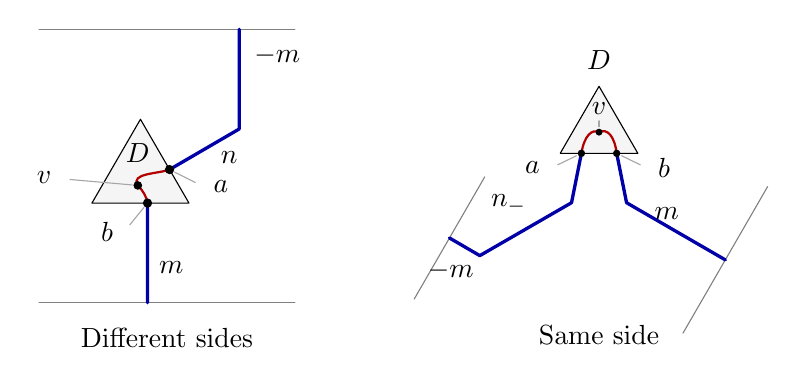
\begin{tikzpicture}[scale=1.12, line cap=round, line join=round,
  arm/.style={very thick,blue!65!black}, chord/.style={thick,red!70!black},
  leader/.style={thin,gray!70,shorten >=2pt,shorten <=1pt}]
\begin{scope}
\draw[gray] (-1.15,-1.45)--(1.75,-1.45);
\draw[gray] (-1.15,1.65)--(1.75,1.65);
\draw[fill=gray!8] (-.55,-.32)--(.55,-.32)--(0,.63)--cycle;
\node at (-.03,.25) {$D$};
\coordinate (a) at (.33,.06); \coordinate (b) at (.08,-.32);
\draw[chord] (a) .. controls (.2,.01) and (-.12,.02) .. (-.03,-.12)
 .. controls (.03,-.18) and (.07,-.25) .. (b);
\fill (-.03,-.12) circle (1.4pt);
\draw[leader] (-.83,-.05)--(-.03,-.12);
\node[anchor=east] at (-.90,-.03) {$v$};
\draw[arm] (b)--(.08,-1.45);
\draw[arm] (a)--(1.12,.52)--(1.12,1.65);
\fill (a) circle (1.5pt);
\draw[leader] (.65,-.10)--(a);
\node[anchor=west] at (.72,-.13) {$a$};
\fill (b) circle (1.5pt);
\draw[leader] (-.14,-.59)--(b);
\node[anchor=east] at (-.20,-.65) {$b$};
\node at (.3,-1.85) {Different sides};
\node[anchor=west] at (1.18,1.35) {$-m$};
\node[anchor=west] at (.1,-1.05) {$m$};
\node[anchor=west] at (.8,.2) {$n$};
\end{scope}
\begin{scope}[xshift=5.2cm,yshift=.5cm,scale=.8]
\coordinate (a) at (-.25,-.32); \coordinate (b) at (.25,-.32);
\draw[gray] (-2.62,-2.386)--(-1.62,-.654);
\draw[gray] (1.19,-2.869)--(2.39,-.791);
\draw[fill=gray!8] (-.55,-.32)--(.55,-.32)--(0,.63)--cycle;
\node[anchor=south] at (0,.73) {$D$};
\draw[chord] (a) .. controls (-.21,-.07) and (-.1,.03) .. (0,-.02)
 .. controls (.12,.04) and (.22,-.08) .. (b);
\fill (0,-.02) circle (1.4pt);
\draw[leader] (0,.18)--(0,-.02);
\node at (0,.32) {$v$};
\draw[arm] (a)--(-.39,-1.02)--(-1.69,-1.77)--(-2.12,-1.52);
\draw[arm] (b)--(.39,-1.02)--(1.79,-1.83);
\fill (a) circle (1.5pt);
\draw[leader] (-.62,-.50)--(a);
\node[anchor=east] at (-.70,-.52) {$a$};
\fill (b) circle (1.5pt);
\draw[leader] (.62,-.50)--(b);
\node[anchor=west] at (.70,-.52) {$b$};
\node at (0,-2.9) {Same side};
\node at (.96,-1.17) {$m$};
\node at (-1.28,-1.04) {$n_-$};
\node at (-2.1,-1.98) {$-m$};
\end{scope}
\end{tikzpicture}

\caption{Exterior-arm layouts, schematically.  The red chord visits the
marked vertex inside the central triangle.  Blue routes leave its incident
sides into the exterior and reach opposite strip walls.  Different sides
require at most one bend on one arm; equal sides use separating initial
rays and at most two bends.  Actual walks occupy narrow neighborhoods of
these routes, with widening first tubes at separated ports.}
\label{fig:exterior-arms}
\end{figure}

In the first layout put \(d=a-b\), where \(a,b\) are the \(A,B\)
ports. Since \(n\cdot d\ge0\), \(m\cdot d\le0\), and
\(n\cdot m=-1/2\), the initial rays satisfy
\[
 |d+yn-t'm|^2\ge |d|^2+y^2+(t')^2+yt'\qquad(y,t'\ge0).
\]
Their separation is therefore at least a constant times \(g+y+t'\). The later \(A\)-arm has macroscopic separation in \(n\)-projection from the \(B\)-ray and from the central \(A\) line, towards its exterior. In the second layout the initial separation in \(t\)-projection is at least \(g+\kappa(y+t')\); thereafter there is macroscopic separation in this projection, with the two arms continuing away from each other (also each later piece is apart from the opposite initial piece). Both beyond their first rays stay macroscopically to the exterior of the \(A\) line: the long \(n_-\) piece moves farther out. The first bend already has
normal depth \(R/8\) outside that line, and the final length \(R/8\)
toward \(-m\) reduces that depth by only \(R/16\). Thus a margin of
at least \(R/16\) remains. The left arm's nonconsecutive pieces are apart in \(t\)-projection. Thus these are uniformly simple routes of the bend type just discussed, with target-wall clearance except at the respective aligned terminal pieces, and we can ensure for the actual paths that each arm stays strictly outside its incident central line and the two are disjoint. Indeed first straight bridges remain strictly exterior to their starting line and opening widths and slope deviations can be made arbitrarily small relative to the displayed initial separation; tiny fixed-proportion bend and tube neighborhoods suffice afterwards. Nominal depths/lengths are comparable to \(R\), with \(c\) small as stipulated, and all subsequent parameter choices for the sewing estimates can be uniform over the central locations and independent of \(\epsilon\).

\paragraph{Normalizing an arm using only its own initial port.}
Fix the ordered side pair, the target strip, and each arm's role once
and for all.  In the equal-side case these roles are left and right along
$t$; otherwise they are the $A$ and $B$ sides.  For a fixed triangle $D$
and role, the route and its permitted narrow neighborhoods depend only
on that arm's own starting port $a$.  The second port is needed only to
verify the separation of the two already chosen neighborhoods.  All tube
widths, bend sizes and terminal windows are chosen uniformly in the
allowed ports and independently of $\epsilon$.

Let $Q_{D,\mathrm{role}}(a)$ be the mass of this one-arm family, with its
terminal port summed over the fixed target window.  The bend estimates
give $Q_{D,\mathrm{role}}(a)\ge R^{-p-K_{\mathrm{loss}}\epsilon}$ for a uniform $K_{\mathrm{loss}}$
and large $R$.  Multiply every weight in this family by
\[
 \lambda_{D,\mathrm{role}}(a)
 =\frac{R^{-p-K_{\mathrm{loss}}\epsilon}}{Q_{D,\mathrm{role}}(a)}\le1.
\]
Its thinned total mass is exactly $R^{-p-K_{\mathrm{loss}}\epsilon}$.  In particular,
this scalar does not depend on the other endpoint of the central chord. Concatenating with the chord gives bridges through \(v\); the central interval is uniquely determined given the triangle by the interior condition and the exterior arm constraints. Over full distinct bridges visiting \(v\) write \(m_D\) for the product of thinning factors when represented for that triple, zero otherwise. Thus
\[
 \sum_\xi w_\xi\sum_D m_D(\xi)\ \ge\ R^{3+z-o(1)-2p-2K_{\mathrm{loss}}\epsilon}.
\]
\paragraph{The two-representation decomposition.}
For two offset triples representing the same bridge the central intervals both contain \(v\) (visited only once). Entry at the more exterior \(A\) line precedes entry at the inner one if distinct (both before \(v\), and the former point cannot be inside the other chord); likewise exits in reverse order at side \(B\). Equal entry or exit offsets give the same corresponding crossing. Overlap between inner crossings is a marked excursion of the intersection triangle, total mass \(\le R^{z+o(1)}\). Segments between crossings at offset gaps \(\Delta_A,\Delta_B\) are strip bridges (within the more exterior chord and the other extension which stays strictly outside its central wall), costing the corresponding \(O((1+\Delta)^{-p})\) given inner ports. Remaining segments are full arms for the respective exterior-crossing representations.  For this second-moment estimate the pair \(D,D'\) is fixed. Select the
representation with the exterior entry crossing and the one with the
exterior exit crossing, making a fixed choice at a tie. These known
representation labels, roles and recovered own initial ports fix the
two arm families and their thinning factors. The two selections may
come from different offset triples. Retain these two factors from \(m_Dm_{D'}\), and drop the unused
factors, which are at most one. Each recovered full arm then costs at most
\(R^{-p}\), by its prescribed thinned total mass.

Figure~\ref{fig:recoverable-cuts} shows a mixed ordering when \(A\ne B\).
It records order along the path; the preceding localization argument is
what makes the marked interval a chord in the intersection triangle.
When \(A=B\), the offset order is the same at entry and exit, so one
triangle supplies both exterior arms. The decomposition still has two
possible gap bridges, now with the same normal width.
\begin{figure}[htbp]
\centering
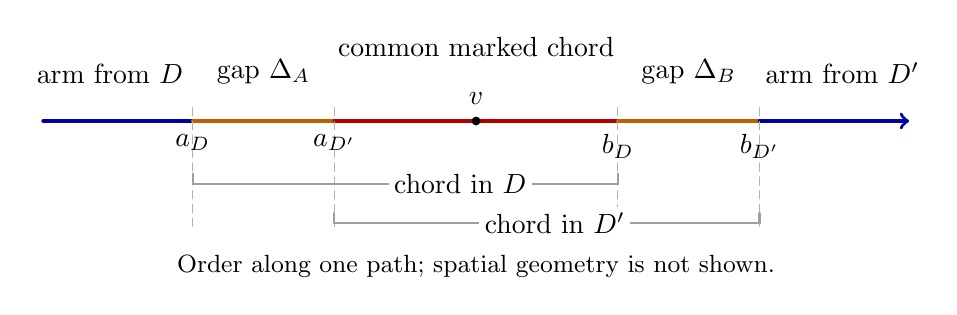
\begin{tikzpicture}[x=1cm,y=1cm,line cap=round,
  arm/.style={very thick,blue!65!black},
  gap/.style={very thick,orange!75!black},
  core/.style={very thick,red!70!black},
  guide/.style={thin,gray!60,densely dashed}]
\draw[arm] (0,0)--(1.9,0);
\draw[gap] (1.9,0)--(3.7,0);
\draw[core] (3.7,0)--(7.3,0);
\draw[gap] (7.3,0)--(9.1,0);
\draw[arm,->] (9.1,0)--(11,0);
\foreach \xx in {1.9,3.7,7.3,9.1}{\draw[guide] (\xx,.17)--(\xx,-1.4);}
\fill (5.5,0) circle (1.6pt);
\node[above] at (5.5,.08) {$v$};
\node[above,align=center] at (.85,.35) {arm from $D$};
\node[above,align=center] at (2.8,.35) {gap $\Delta_A$};
\node[above,align=center] at (5.5,.7) {common marked chord};
\node[above,align=center] at (8.2,.35) {gap $\Delta_B$};
\node[above,align=center] at (10.15,.35) {arm from $D'$};
\node[below] at (1.9,-.05) {$a_D$};
\node[below] at (3.7,-.05) {$a_{D'}$};
\node[below] at (7.3,-.05) {$b_D$};
\node[below] at (9.1,-.05) {$b_{D'}$};
\draw[thick,gray!75] (1.9,-.67)--(1.9,-.8)--(7.3,-.8)--(7.3,-.67);
\node[fill=white,inner sep=2pt] at (5.3,-.8) {chord in $D$};
\draw[thick,gray!75] (3.7,-1.17)--(3.7,-1.3)--(9.1,-1.3)--(9.1,-1.17);
\node[fill=white,inner sep=2pt] at (6.5,-1.3) {chord in $D'$};
\node[align=center,font=\small] at (5.5,-1.85)
 {Order along one path; spatial geometry is not shown.};
\end{tikzpicture}

\caption{Two representations of one bridge, shown in path order. In this
mixed ordering the exterior entry comes from \(D\) and the exterior exit
from \(D'\). The inner crossings delimit the marked chord in
\(D\cap D'\); the adjacent pieces cross the two parallel cut gaps.
The remaining ends are complete arms from the indicated representations.
The drawing asserts no spatial monotonicity of the path.}
\label{fig:recoverable-cuts}
\end{figure}

The joint second moment bound is
\[
 \sum_\xi w_\xi\big(\sum_D m_D(\xi)\big)^2
 \le R^{6+z+o(1)-4p}.
\]
Here is the offset sum in both cases. If \(A\ne B\), the two used
side offsets vary independently and each has
\[
 \sum_{d,d'}(1+|d-d'|)^{-p}=O(R^{2-p}).
\]
The unused side gives \(O(R^2)\) further pairs. If \(A=B\), the two gaps
coincide, and instead
\[
 \sum_{d,d'}(1+|d-d'|)^{-2p}=O(R^{2-2p}),
\]
while the other two side offsets give \(O(R^4)\) pairs. The latter sum
uses \(2p<1\). Thus in either case the offset sum is \(O(R^{6-2p})\).
The marked chord and the two normalized exterior arms supply the remaining
factor \(R^{z-2p+o(1)}\), proving the second-moment bound.

Apply \eqref{eq:sewing-cauchy} to obtain distinct bridge mass through
\(v\) at least \(R^{z-4K_{\mathrm{loss}}\epsilon-o(1)}\). Sum this for \(\asymp R^2\) vertices \(v\), with only boundedly many oriented strip choices and \(O(R)\) starting ports total; use lattice symmetry to translate to standard strip bridges from a fixed port. This proves the confined length-sum lower of \eqref{c2:eq-E1}, since
$\epsilon$ was arbitrary.  The constant $K_{\mathrm{loss}}$ affects only the
exponent.  The corridor width was fixed by the layouts and tube widths
independently of $\epsilon$, so letting $\epsilon\downarrow0$ keeps one fixed
corridor.

For the upper, in convex bounded truncations of the strip the positive mass of bridges through any vertex \(v\), allowing all starts, is at most \(C T_v\) by \eqref{c2:eq-1}. Uniformly \(T_v\le R^{z+o(1)}\) by \eqref{c2:eq-G3}: polygons around an incident face with dyadic diameter \(L\ge R\) cost only \(O(R/L)\) total mass in each such dyad, by Proposition~\ref{prop:adjacent-bridges-shapes} and at most \(O(RL)\) translations per shape (normal translation strip-constrained, lateral shift limited by enclosure). The large loops thus cost bounded partition factor and the others are in a ball of order \(R\) for \eqref{c2:eq-G1}. Exhaust to count all finite bridges. To make the last translation count explicit, let \(\mathcal F_R\) be
one set of vertex representatives in the strip modulo translation by
\(U\), and let \(A_R(v)\) be the positive mass of bridges through \(v\)
with the bottom starting port also summed. Then
\[
 M(R)=\sum_{v\in\mathcal F_R}A_R(v),\qquad |\mathcal F_R|=O(R).
\]
Indeed translate a bridge with one marked visited vertex so that its
starting port is the fixed standard port. Conversely a bridge from that
port, together with any one of its vertices, has a unique translate that
places the marked vertex in \(\mathcal F_R\). All weights are preserved.
The bound \(A_R(v)\le R^{z+o(1)}\) therefore proves the upper bound in
\eqref{c2:eq-E1}.



We can now assemble Theorem~\ref{thm:confined-bridge}. The lateral tightness
proved at the start of this section makes \(B(R)-B_C(R)\) an arbitrarily
small fixed fraction of \(B(R)\) when the fixed constant \(C\) is large.
Together with the boundary estimate, this gives
\(B_C(R)\asymp B(R)\asymp R^{-1/4}\). The two-arm construction gives the
confined first-moment lower bound with a corridor constant independent of
\(\epsilon\); the preceding upper bound and \(M_C(R)\le M(R)\) give
both \(M_C(R)=R^{13/12+o(1)}\) and \(M(R)=R^{13/12+o(1)}\). Dividing either first moment by
its corresponding mass yields the mean exponent \(13/12+1/4=4/3\).
